%!TEX TS-program = xelatex
\documentclass[10pt,oneside]{article}

\usepackage[english]{babel}

\usepackage{amsmath,amssymb,amsfonts}
\usepackage[utf8]{inputenc}
\usepackage[T1]{fontenc}
\usepackage{stix}
\usepackage[scaled]{helvet}
\usepackage[scaled]{inconsolata}

\usepackage{lastpage}

\usepackage{setspace}

\usepackage{ccicons}

\usepackage[hang,flushmargin]{footmisc}

\usepackage{geometry}

\setlength{\parindent}{0pt}
\setlength{\parskip}{6pt plus 2pt minus 1pt}

\usepackage{fancyhdr}
\renewcommand{\headrulewidth}{0pt}\providecommand{\tightlist}{%
  \setlength{\itemsep}{0pt}\setlength{\parskip}{0pt}}

\makeatletter
\newcounter{tableno}
\newenvironment{tablenos:no-prefix-table-caption}{
  \caption@ifcompatibility{}{
    \let\oldthetable\thetable
    \let\oldtheHtable\theHtable
    \renewcommand{\thetable}{tableno:\thetableno}
    \renewcommand{\theHtable}{tableno:\thetableno}
    \stepcounter{tableno}
    \captionsetup{labelformat=empty}
  }
}{
  \caption@ifcompatibility{}{
    \captionsetup{labelformat=default}
    \let\thetable\oldthetable
    \let\theHtable\oldtheHtable
    \addtocounter{table}{-1}
  }
}
\makeatother

\usepackage{array}
\newcommand{\PreserveBackslash}[1]{\let\temp=\\#1\let\\=\temp}
\let\PBS=\PreserveBackslash

\usepackage[breaklinks=true]{hyperref}
\hypersetup{colorlinks,%
citecolor=blue,%
filecolor=blue,%
linkcolor=blue,%
urlcolor=blue}
\usepackage{url}

\usepackage{caption}
\setcounter{secnumdepth}{0}
\usepackage{cleveref}

\usepackage{graphicx}
\makeatletter
\def\maxwidth{\ifdim\Gin@nat@width>\linewidth\linewidth
\else\Gin@nat@width\fi}
\makeatother
\let\Oldincludegraphics\includegraphics
\renewcommand{\includegraphics}[1]{\Oldincludegraphics[width=\maxwidth]{#1}}

\usepackage{longtable}
\usepackage{booktabs}

\usepackage{color}
\usepackage{fancyvrb}
\newcommand{\VerbBar}{|}
\newcommand{\VERB}{\Verb[commandchars=\\\{\}]}
\DefineVerbatimEnvironment{Highlighting}{Verbatim}{commandchars=\\\{\}}
% Add ',fontsize=\small' for more characters per line
\usepackage{framed}
\definecolor{shadecolor}{RGB}{248,248,248}
\newenvironment{Shaded}{\begin{snugshade}}{\end{snugshade}}
\newcommand{\KeywordTok}[1]{\textcolor[rgb]{0.13,0.29,0.53}{\textbf{#1}}}
\newcommand{\DataTypeTok}[1]{\textcolor[rgb]{0.13,0.29,0.53}{#1}}
\newcommand{\DecValTok}[1]{\textcolor[rgb]{0.00,0.00,0.81}{#1}}
\newcommand{\BaseNTok}[1]{\textcolor[rgb]{0.00,0.00,0.81}{#1}}
\newcommand{\FloatTok}[1]{\textcolor[rgb]{0.00,0.00,0.81}{#1}}
\newcommand{\ConstantTok}[1]{\textcolor[rgb]{0.00,0.00,0.00}{#1}}
\newcommand{\CharTok}[1]{\textcolor[rgb]{0.31,0.60,0.02}{#1}}
\newcommand{\SpecialCharTok}[1]{\textcolor[rgb]{0.00,0.00,0.00}{#1}}
\newcommand{\StringTok}[1]{\textcolor[rgb]{0.31,0.60,0.02}{#1}}
\newcommand{\VerbatimStringTok}[1]{\textcolor[rgb]{0.31,0.60,0.02}{#1}}
\newcommand{\SpecialStringTok}[1]{\textcolor[rgb]{0.31,0.60,0.02}{#1}}
\newcommand{\ImportTok}[1]{#1}
\newcommand{\CommentTok}[1]{\textcolor[rgb]{0.56,0.35,0.01}{\textit{#1}}}
\newcommand{\DocumentationTok}[1]{\textcolor[rgb]{0.56,0.35,0.01}{\textbf{\textit{#1}}}}
\newcommand{\AnnotationTok}[1]{\textcolor[rgb]{0.56,0.35,0.01}{\textbf{\textit{#1}}}}
\newcommand{\CommentVarTok}[1]{\textcolor[rgb]{0.56,0.35,0.01}{\textbf{\textit{#1}}}}
\newcommand{\OtherTok}[1]{\textcolor[rgb]{0.56,0.35,0.01}{#1}}
\newcommand{\FunctionTok}[1]{\textcolor[rgb]{0.00,0.00,0.00}{#1}}
\newcommand{\VariableTok}[1]{\textcolor[rgb]{0.00,0.00,0.00}{#1}}
\newcommand{\ControlFlowTok}[1]{\textcolor[rgb]{0.13,0.29,0.53}{\textbf{#1}}}
\newcommand{\OperatorTok}[1]{\textcolor[rgb]{0.81,0.36,0.00}{\textbf{#1}}}
\newcommand{\BuiltInTok}[1]{#1}
\newcommand{\ExtensionTok}[1]{#1}
\newcommand{\PreprocessorTok}[1]{\textcolor[rgb]{0.56,0.35,0.01}{\textit{#1}}}
\newcommand{\AttributeTok}[1]{\textcolor[rgb]{0.77,0.63,0.00}{#1}}
\newcommand{\RegionMarkerTok}[1]{#1}
\newcommand{\InformationTok}[1]{\textcolor[rgb]{0.56,0.35,0.01}{\textbf{\textit{#1}}}}
\newcommand{\WarningTok}[1]{\textcolor[rgb]{0.56,0.35,0.01}{\textbf{\textit{#1}}}}
\newcommand{\AlertTok}[1]{\textcolor[rgb]{0.94,0.16,0.16}{#1}}
\newcommand{\ErrorTok}[1]{\textcolor[rgb]{0.64,0.00,0.00}{\textbf{#1}}}
\newcommand{\NormalTok}[1]{#1}

\newlength{\cslhangindent}
\setlength{\cslhangindent}{1.5em}
\newlength{\csllabelwidth}
\setlength{\csllabelwidth}{3em}
\newenvironment{CSLReferences}[3] % #1 hanging-ident, #2 entry spacing
 {% don't indent paragraphs
  \setlength{\parindent}{0pt}
  % turn on hanging indent if param 1 is 1
  \ifodd #1 \everypar{\setlength{\hangindent}{\cslhangindent}}\ignorespaces\fi
  % set entry spacing
  \ifnum #2 > 0
  \setlength{\parskip}{#2\baselineskip}
  \fi
 }%
 {}
\usepackage{calc} % for \widthof, \maxof
\newcommand{\CSLBlock}[1]{#1\hfill\break}
\newcommand{\CSLLeftMargin}[1]{\parbox[t]{\maxof{\widthof{#1}}{\csllabelwidth}}{#1}}
\newcommand{\CSLRightInline}[1]{\parbox[t]{\linewidth}{#1}}
\newcommand{\CSLIndent}[1]{\hspace{\cslhangindent}#1}\usepackage[table,dvipsnames]{xcolor}

\geometry{includemp,
            letterpaper,
            top=1.2in,
            bottom=2.510cm,
            inner=0.5in,
            outer=0.4in,
            marginparwidth=1.95in,
            marginparsep=0.4in}

\usepackage[singlelinecheck=off]{caption}
\captionsetup{
  font={small},
  labelfont={bf},
  format=plain,
  labelsep=quad
}
\usepackage{floatrow}
\floatsetup[figure]{margins=hangright,
              facing=no,
              capposition=beside,
              capbesideposition={center,outside},
              floatwidth=\textwidth}
\floatsetup[table]{margins=hangoutside,
             facing=yes,
             capposition=beside,
             capbesideposition={center,outside},
             floatwidth=\textwidth}

\pagestyle{plain}

\setcounter{secnumdepth}{5}

\usepackage{titlesec}

\titleformat{\section}[block]
{\normalfont\large\sffamily}
{\thesection}{.5em}{\titlerule\\[.8ex]\bfseries}

\titleformat{\subsection}[runin]
{\normalfont\fontseries{b}\selectfont\filright\sffamily}
{\thesubsection.}{.5em}{}

\titleformat{\subsubsection}[runin]
{\normalfont\itshape\rmfamily\bfseries}{\thesubsubsection}{1em}{}

\fancypagestyle{firstpage}
{
   \fancyhf{}
   \renewcommand{\headrulewidth}{0pt}
   \fancyfoot[R]{\footnotesize\ccby}
   \fancyfoot[L]{\footnotesize\sffamily\today}
}

\fancypagestyle{normal}
{
  \fancyhf{}
  \fancyfoot[R]{\footnotesize\sffamily\thepage\ of \pageref*{LastPage}}
}

\usepackage{tikz}
\begin{document}
\tikz [remember picture, overlay] %
\node [shift={(-0.6in,1.1cm)},scale=0.2,opacity=0.4] at (current page.south east)[anchor=south east]{
\includegraphics{logo}};%
\pagestyle{normal}
\thispagestyle{firstpage}

\newcommand{\colorRule}[3][black]{\textcolor[HTML]{#1}{\rule{#2}{#3}}}

\noindent {\LARGE \textbf{\textsf{Food web reconstruction through
phylogenetic transfer of low-rank network representation}}}

\medskip
\begin{flushleft}
{\small
%
\href{https://orcid.org/0000-0001-6067-1349}{Tanya\,Strydom}%
%
\,\textsuperscript{1,2,‡}, %
\href{https://orcid.org/0000-0003-0193-5441}{Salomé\,Bouskila}%
%
\,\textsuperscript{1,‡}, %
\href{https://orcid.org/0000-0001-9051-0597}{Francis\,Banville}%
%
\,\textsuperscript{1,3,2}, %
\href{https://orcid.org/0000-0003-4036-977X}{Ceres\,Barros}%
%
\,\textsuperscript{4}, %
\href{https://orcid.org/0000-0002-2151-6693}{Dominique\,Caron}%
%
\,\textsuperscript{5,2}, %
\href{https://orcid.org/0000-0003-0452-6993}{Maxwell J\,Farrell}%
%
\,\textsuperscript{6}, %
\href{https://orcid.org/0000-0002-9935-1366}{Marie-Josée\,Fortin}%
%
\,\textsuperscript{6}, %
\href{https://orcid.org/0000-0003-3220-6161}{Victoria\,Hemming}%
%
\,\textsuperscript{4}, %
\href{https://orcid.org/0000-0002-4104-9463}{Benjamin\,Mercier}%
%
\,\textsuperscript{3,2}, %
\href{https://orcid.org/0000-0002-6004-4027}{Laura J.\,Pollock}%
%
\,\textsuperscript{5}, %
\href{https://orcid.org/0000-0001-5785-8321}{Rogini\,Runghen}%
%
\,\textsuperscript{7}, %
\href{https://orcid.org/0000-0002-3454-0633}{Giulio V.\,Dalla Riva}%
%
\,\textsuperscript{8}, %
\href{https://orcid.org/0000-0002-0735-5184}{Timothée\,Poisot}%
%
\,\textsuperscript{1,2}
\vskip 1em
\textsuperscript{1}\,Département de Sciences Biologiques, Université de
Montréal, Montréal, Canada; \textsuperscript{2}\,Québec Centre for
Biodiversity Sciences, Montréal, Canada; \textsuperscript{3}\,Université
de Sherbrooke, Sherbrooke, Canada; \textsuperscript{4}\,Department of
Forest Resources Management, University of British Columbia, Vancouver,
Canada; \textsuperscript{5}\,Department of Biology, McGill University,
Montréal, Canada; \textsuperscript{6}\,Department of Ecology \&
Evolutionary Biology, University of Toronto, Toronto,
Canada; \textsuperscript{7}\,Centre for Integrative Ecology, School of
Biological Sciences, University of Canterbury, Canterbury, New
Zealand; \textsuperscript{8}\,School of Mathematics and Statistics,
University of Canterbury, Canterbury, New Zealand\\
\textsuperscript{‡}\,These authors contributed equally to the work\\
\vskip 1em
\textbf{Correspondance to:}\\
Timothée Poisot --- \texttt{timothee.poisot@umontreal.ca}\\
}
\end{flushleft}

\vskip 2em
\makebox[0pt][l]{\colorRule[CCCCCC]{2.0\textwidth}{0.5pt}}
\vskip 2em
\noindent

\marginpar{\vskip 1em\flushright
{\small{\bfseries Keywords}:\par
ecological networks\\network embedding\\transfer learning\\ancestral
character estimation\\biogeography\\}
}


\textbf{Abstract}:\,Despite their importance in many ecological
processes, collecting data and information on ecological interactions,
and therefore species interaction networks, is an exceedingly
challenging task. For this reason, large parts of the world have a
deficit of data of which species interact, and what we can expect the
network structure of these interactions to be. As data collection alone
is unlikely to be sufficient at filling these global gaps, community
ecologists must adopt predictive methods. In this contribution we
develop such a method, relying on graph embedding (the extraction of
explanatory latent variables from known graph structures) and transfer
learning (the application of previous solution to novel problems with
limited predictors overlap) in order to assemble a predicted list of
trophic interactions between mammals of Canada. This interaction list is
derived from extensive knowledge of the mammalian food web of Europe,
despite the fact that there are fewer than 5\% of common species between
the two locations. We provide guidance on how this method can be adapted
by substituting some approaches or predictors in order to make it more
generally applicable to a broad family of ecological problems.

\vskip 2em
\makebox[0pt][l]{\colorRule[CCCCCC]{2.0\textwidth}{0.5pt}}
\vskip 2em

\hypertarget{introduction}{%
\section{Introduction}\label{introduction}}

There are two core challenges we are faced with in furthering our
understanding of ecological networks across space, particularly at
macro-ecologically relevant scales (\emph{e.g.} Trøjelsgaard and Olesen
2016). First, networks within a location are difficult to sample
properly (Jordano 2016a, 2016b), resulting in a widespread ``Eltonian
shortfall'' (Hortal et al. 2015). This first challenge (local
incompleteness) has been, in large part, addressed by the recent
multiplication of methods aiming to predict interactions \emph{within}
an \emph{existing} network, a lot of which are reviewed in Strydom et
al. (2021). Second, recent analyses based on collected data (Poisot,
Bergeron, et al. 2021) or metadata (Cameron et al. 2019) highlight that
ecological networks are currently studied in a biased subset of space
and bioclimates, which impedes our ability to generalize any local
understanding of network structure. Meaning that although the framework
to address incompleteness \emph{within} a network exists there would
still be regions that, due to a \emph{lack} of local interaction data,
we are unable to infer potential species interactions. Having a general
solution for the issue of metaweb inference (Morales-Castilla et al.
2015) that, despite situations where minimal knowledge about
interactions within a species pool is known, is capable of producing a
plausible metaweb could be the catalyst for significant breakthroughs in
our ability to start thinking about species interactions networks over
large spatial scales.

Here, we present a general method for the transfer learning of network
representations, relying on the similarities of species in a
biologically/ecologically relevant proxy space (\emph{e.g.} shared
morphology or ancestry). Transfer learning is a machine learning
methodology that uses the knowledge gained from solving one problem and
applying it to a related (destination) problem (Torrey and Shavlik 2010;
Pan and Yang 2010). In this instance, we solve the problem of predicting
trophic interactions between species, based on knowledge extracted from
another species pool for which interactions are known, using
phylogenetic structure as a medium for transfer. This allows us to
construct a \emph{probabilistic} metaweb for a community for which we
have \emph{no} prior interaction data for the desired species pool. Our
methodology is outlined in fig.~\ref{fig:concept}, where we provide an
illustration based on learning an embedding of a metaweb of trophic
interactions for European mammals (known interactions; Maiorano et al.
2020b, 2020a), and based on phylogenetic relationships between mammals
globally (Upham, Esselstyn, and Jetz 2019), infer a metaweb for the
Canadian mammalian species pool (interactions are treated as unknown in
this instance).

\begin{figure}
\hypertarget{fig:concept}{%
\centering
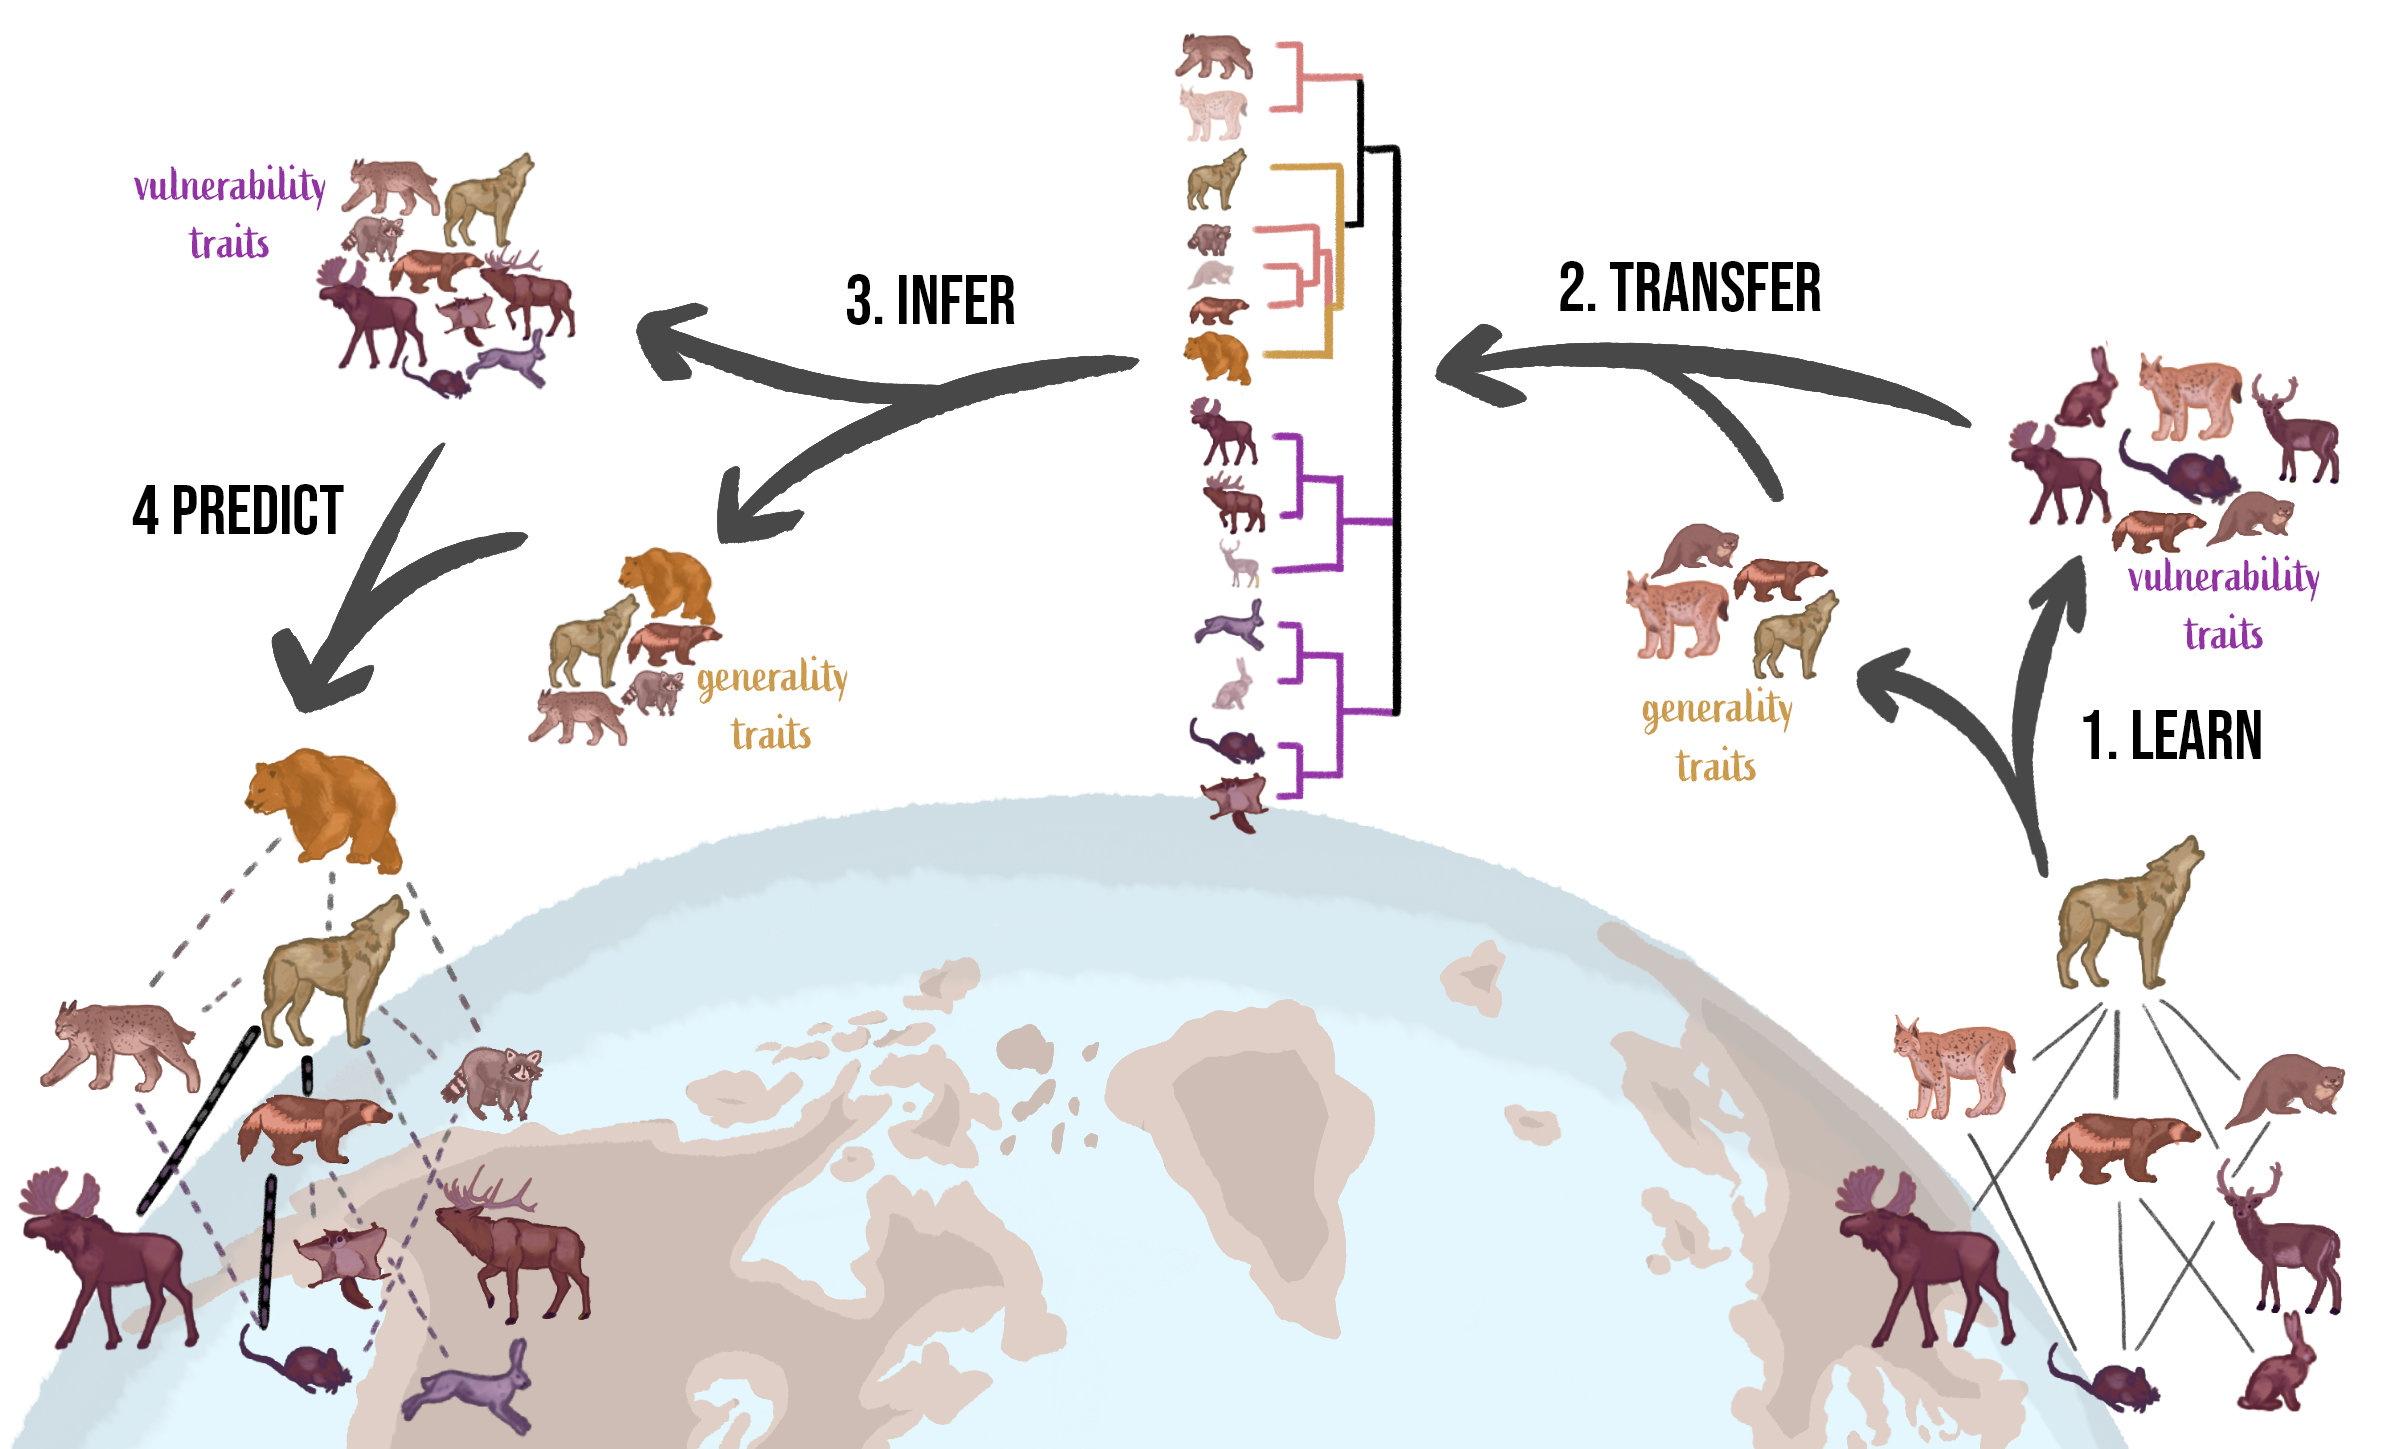
\includegraphics{figures/figure-concept.png}
\caption{Overview of the phylogenetic transfer learning (and prediction)
of species interactions networks. Starting from an initial, known,
network, we learn its representation through a graph embedding step
(here, a truncated Singular Value Decomposition; Step 1), yielding a
series of latent traits (vulnerability traits representing species at
the lower trophic-level and generality traits representing species at
higher trophic-levels; \emph{sensu} Schoener (1989)); second, for the
destination species pool, we perform ancestral character estimation
using a phylogeny (here, using a Brownian model for the latent traits;
Step 2); we then sample from the reconstructed distribution of latent
traits (Step 3) to generate a probabilistic metaweb at the destination
(here, assuming a uniform distribution of traits), and threshold it to
yield the final list of interactions (Step 4).}\label{fig:concept}
}
\end{figure}

There is a plurality of measures of species similarities that can be
used for metaweb reconstruction (see \emph{e.g.} Morales-Castilla et al.
2015); however, phylogenetic proximity has several desirable properties
when working at large scales. Gerhold et al. (2015) made the point that
phylogenetic signal captures diversification of characters (large
macro-evolutionary process), but not necessarily community assembly
(fine ecological process); Dormann et al. (2010) previously found very
similar conclusions. Interactions tend to conserve a phylogenetic signal
that encompasses a wide range of ecological and evolutionary mechanisms
(Mouquet et al. 2012; Cavender-Bares et al. 2009), and - most
importantly - retain this signal even when it is not detectable at the
community scale (Poisot and Stouffer 2018; Hutchinson, Cagua, and
Stouffer 2017). Finally, species interactions at macro-ecological scales
seem to respond mostly to macro-evolutionary processes (Price 2003);
which is evidenced by the presence of conserved backbones in food webs
(Dalla Riva and Stouffer 2016), strong evolutionary signature on prey
choice (Stouffer et al. 2012), and strong phylogenetic signature in food
web intervality (Eklöf and Stouffer 2016). Phylogenetic reconstruction
has also previously been used to understand ancestral plant-insect
interaction networks (Braga et al. 2021). Taken together, these
considerations suggest that phylogenies can reliably be used to transfer
knowledge on species interactions.

Our case study shows that phylogenetic transfer learning is indeed an
effective approach to predict the Canadian mammalian metaweb. This
showcases that although the components (species) that make up the
Canadian and European communities may not be \emph{perfectly} shared, if
the medium (proxy space) selected in the transfer step is biologically
plausible, we can still effectively learn from the known network and
make biologically relevant predictions of interactions. It should be
reiterated that the framework presented in fig.~\ref{fig:concept} is
amenable to changes; notably, the measure of similarity may not be
phylogeny, and can be replaced by information on foraging (Beckerman,
Petchey, and Warren 2006), cell-level mechanisms (Boeckaerts et al.
2021), or a combination of traits and phylogenetic structure (Stock
2021).

\hypertarget{data-used-for-the-case-study}{%
\section{Data used for the case
study}\label{data-used-for-the-case-study}}

We use data on the European metaweb assembled by Maiorano et al.
(2020b), following the definition of the metaweb first introduced by
Dunne (2006), \emph{i.e.} an inventory of all possible interactions
within species from a spatially delimited pool. Notably the metaweb is
not a prediction of the food web at any specific locale within the
frontiers of the species pool -- in fact, these local food webs are
expected to have a subset of both the species and the interactions of
their metaweb (Poisot et al. 2012). This being said, as the metaweb
represents the total of functional, phylogenetic, and macroecological
processes (Morales-Castilla et al. 2015), it is thus still worthy of
ecological attention. We induced the subgraph corresponding to all
mammals by matching species names in the original network first to the
GBIF taxonomic backbone (GBIF Secretariat 2021) and retaining all those
who matched to mammals; all nodes had valid matches to GBIF at this
step, and so this backbone is used for all name reconciliation steps as
outlined below.

The European metaweb represents the knowledge we want to learn and
transfer; the phylogenetic similarity of mammals here represents the
support for transfer. We used the mammalian consensus supertree by
Upham, Esselstyn, and Jetz (2019), for which all approximatively 6000
names have been similarly matched to their GBIF valid names. This step
allows us to place each node of the mammalian European metaweb in the
phylogeny.

The destination problem to which we want to transfer knowledge is the
trophic interactions between mammals in Canada. We obtained the list of
extant species from the IUCN checklist, and selected the terrestrial and
semi-aquatic species (this corresponds to the same selection that was
applied by Maiorano et al. (2020b) in the European metaweb). The IUCN
names were, as previously, reconciled against GBIF to have an exact
match to the taxonomy.

After taxonomic cleaning and reconciliation as outlined in the following
sections, the mammalian European metaweb had 260 species, and the
Canadian species pool has 163; of these, 17 (about 4\% of the total) are
shared, and 89 species from Canada (54\%) had at least one congeneric
species in Europe. The similarity for both species pool predictably
increases with higher taxonomic order, with 19\% of shared genera, 47\%
of shared families, and 75\% of shared orders; for the last point,
Canada and Europe each had a single unique order (\emph{Didelphimorphia}
for Canada, \emph{Erinaceomorpha} for Europe).

In the following sections, we describe the representational learning
step applied to European data, the transfer step through phylogenetic
similarity, and the generation of a probabilistic metaweb for the
destination species pool.

\hypertarget{method-description}{%
\section{Method description}\label{method-description}}

The crux of the method is the transfer of knowledge of a known network,
in order to predict interactions between species from another location.
In fig.~\ref{fig:concept}, we give a high-level overview of the
approach; in the example around which this manuscript is built
(leveraging detailed knowledge about binary trophic interactions between
Mammalia in Europe to predict the less known trophic interactions
between closely phylogenetically related Mammalia in Canada), we use a
series of specific steps for network embedding, trait inference, network
prediction and thresholding.

Specifically, our approach can be summarized as follows: from the known
network in Europe, we use a truncated Singular Value Decomposition
(t-SVD; Halko, Martinsson, and Tropp 2011) to generate latent traits
representing a low-dimensional embedding of the network; these traits
give an unbiased estimate of the node's position in the latent feature
spaces. Then, we map these latent traits onto a reference phylogeny
(other distance-based measures of species proximity that allow for the
inference of features in the latent space can be used, for example the
dissimilarity in functional traits). Based on the reconstructed latent
traits for species in the destination species pool, a Random Dot Product
Graph model (hereafter RDPG; S. J. Young and Scheinerman 2007) predicts
the interaction between species through a function of the nodes'
features through matrix multiplication. Thus, from latent traits and
nodes position, we can infer interactions.

\hypertarget{implementation-and-code-availability}{%
\subsection{Implementation and code
availability}\label{implementation-and-code-availability}}

The entire pipeline is implemented in \emph{Julia} 1.6 (Bezanson et al.
2017) and is available under the permissive MIT License at
\href{https://osf.io/2zwqm/}{\texttt{https://osf.io/2zwqm/}}. The
taxonomic cleanup steps are done using \texttt{GBIF.jl} (Dansereau and
Poisot 2021). The network embedding and analysis is done using
\texttt{EcologicalNetworks.jl} (Banville, Vissault, and Poisot 2021;
Poisot et al. 2019). The phylogenetic simulations are done using
\texttt{PhyloNetworks.jl} (Solís-Lemus, Bastide, and Ané 2017) and
\texttt{Phylo.jl} (Reeve et al. 2016). A complete \texttt{Project.toml}
file specifying the full tree of dependencies is available alongside the
code. This material also includes a fully annotated copy of the entire
code required to run this project (describing both the intent of the
code and discussing some technical implementation details), a vignette
for every step of the process, and a series of Jupyter notebooks with
the text and code. The pipeline can be executed on a laptop in a matter
of minutes, and therefore does not require extensive computational
power.

\hypertarget{step-1-learning-the-origin-network-representation}{%
\subsection{Step 1: Learning the origin network
representation}\label{step-1-learning-the-origin-network-representation}}

The first step in transfer learning is to learn the structure of the
original dataset. In order to do so, we rely on an approach inspired
from representational learning, where we learn a \emph{representation}
of the metaweb (in the form of the latent subspaces), rather than a list
of interactions (species \emph{a} eats \emph{b}). This approach is
conceptually different from other metaweb-scale predictions
(\emph{.e.g.} Albouy et al. 2019), in that the metaweb representation is
easily transferable. Specifically, we use RDPG to create a number of
latent variables that can be combined into an approximation of the
network adjacency matrix. RDPG results are known to have strong
phylogenetic signal, and to capture the evolutionary backbone of food
webs (Dalla Riva and Stouffer 2016). In addition, recent advances show
that the latent variables produced this way can be used to predict
\emph{de novo} network edges (Runghen, Stouffer, and Dalla Riva 2021).

The latent variables are created by performing a truncated Singular
Value Decomposition (t-SVD) on the adjacency matrix. SVD is an
appropriate embedding of ecological networks, which has recently been
shown to both capture their complex, emerging properties (Strydom, Dalla
Riva, and Poisot 2021) and to allow highly accurate prediction of the
interactions within a single network (Poisot, Ouellet, et al. 2021).
Under SVD, an adjacency matrix \(\mathbf{A}\) (where
\(\mathbf{A}_{m,n}\in\mathbb{B}\) where 1 indicates predation and 0 an
absence thereof) is decomposed into three components resulting in
\(\mathbf{A} = \mathbf{L}\mathbf{\Sigma}\mathbf{R}.\) Here,
\(\mathbf{\Sigma}\) is a \(m \times n\) diagonal matrix and contains
only singular (\(\sigma\)) values along its diagonal, \(\mathbf{L}\) is
a \(m \times m\) unitary matrix, and \(\mathbf{R}'\) a \(n \times n\)
unitary matrix. Truncating the SVD removes additional noise in the
dataset by omitting non-zero and/or smaller \(\sigma\) values from
\(\mathbf{\Sigma}\) using the rank of the matrix. Under a t-SVD
\(\mathbf{A}_{m,n}\) is decomposed so that \(\mathbf{\Sigma}\) is a
square \(r \times r\) diagonal matrix (where \(r\) is the rank of
\(\mathbf{A}\)) containing only non-zero \(\sigma\) values.
Additionally, \(\mathbf{L}\) is now a \(m \times r\) semi unitary matrix
and \(\mathbf{R}'\) a \(n \times r\) semi-unitary matrix.

The specific rank at which the SVD ought to be truncated is a difficult
question. The purpose of SVD is to remove the noise (expressed at high
dimensions) and to focus on the signal, (expressed at low dimensions).
In datasets with a clear signal/noise demarcation, a scree plot of
\(\mathbf{\Sigma}\) can show a sharp drop at the rank where noise starts
(Zhu and Ghodsi 2006). Because the European metaweb is almost entirely
known, the amount of noise is low; this is reflected in
fig.~\ref{fig:scree} (left), where the scree plot shows no important
drop, and in fig.~\ref{fig:scree} (right) where the proportion of
variance explained increases smoothly at higher dimensions. For this
reason, we default back to an arbitrary threshold that explains 60\% of
the variance in the underlying data, corresponding to 12 dimensions.

A RDPG estimates the probability of observing interactions between nodes
(species) as a function of the nodes' latent variables. The latent
variables used for the RDPG, called the left and right subspaces, are
defined as \(\mathcal{L} = \mathbf{L}\sqrt{\mathbf{\Sigma}}\), and
\(\mathcal{R} = \sqrt{\mathbf{\Sigma}}\mathbf{R}\) -- using the full
rank of \(\mathbf{A}\), \(\mathcal{L}\mathcal{R}' = \mathbf{A}\), and
using any smaller rank results in
\(\mathcal{L}\mathcal{R}' \approx \mathbf{A}\). Using a rank of 1 for
the t-SVD provides a first-order approximation of the network.

\begin{figure}
\hypertarget{fig:scree}{%
\centering
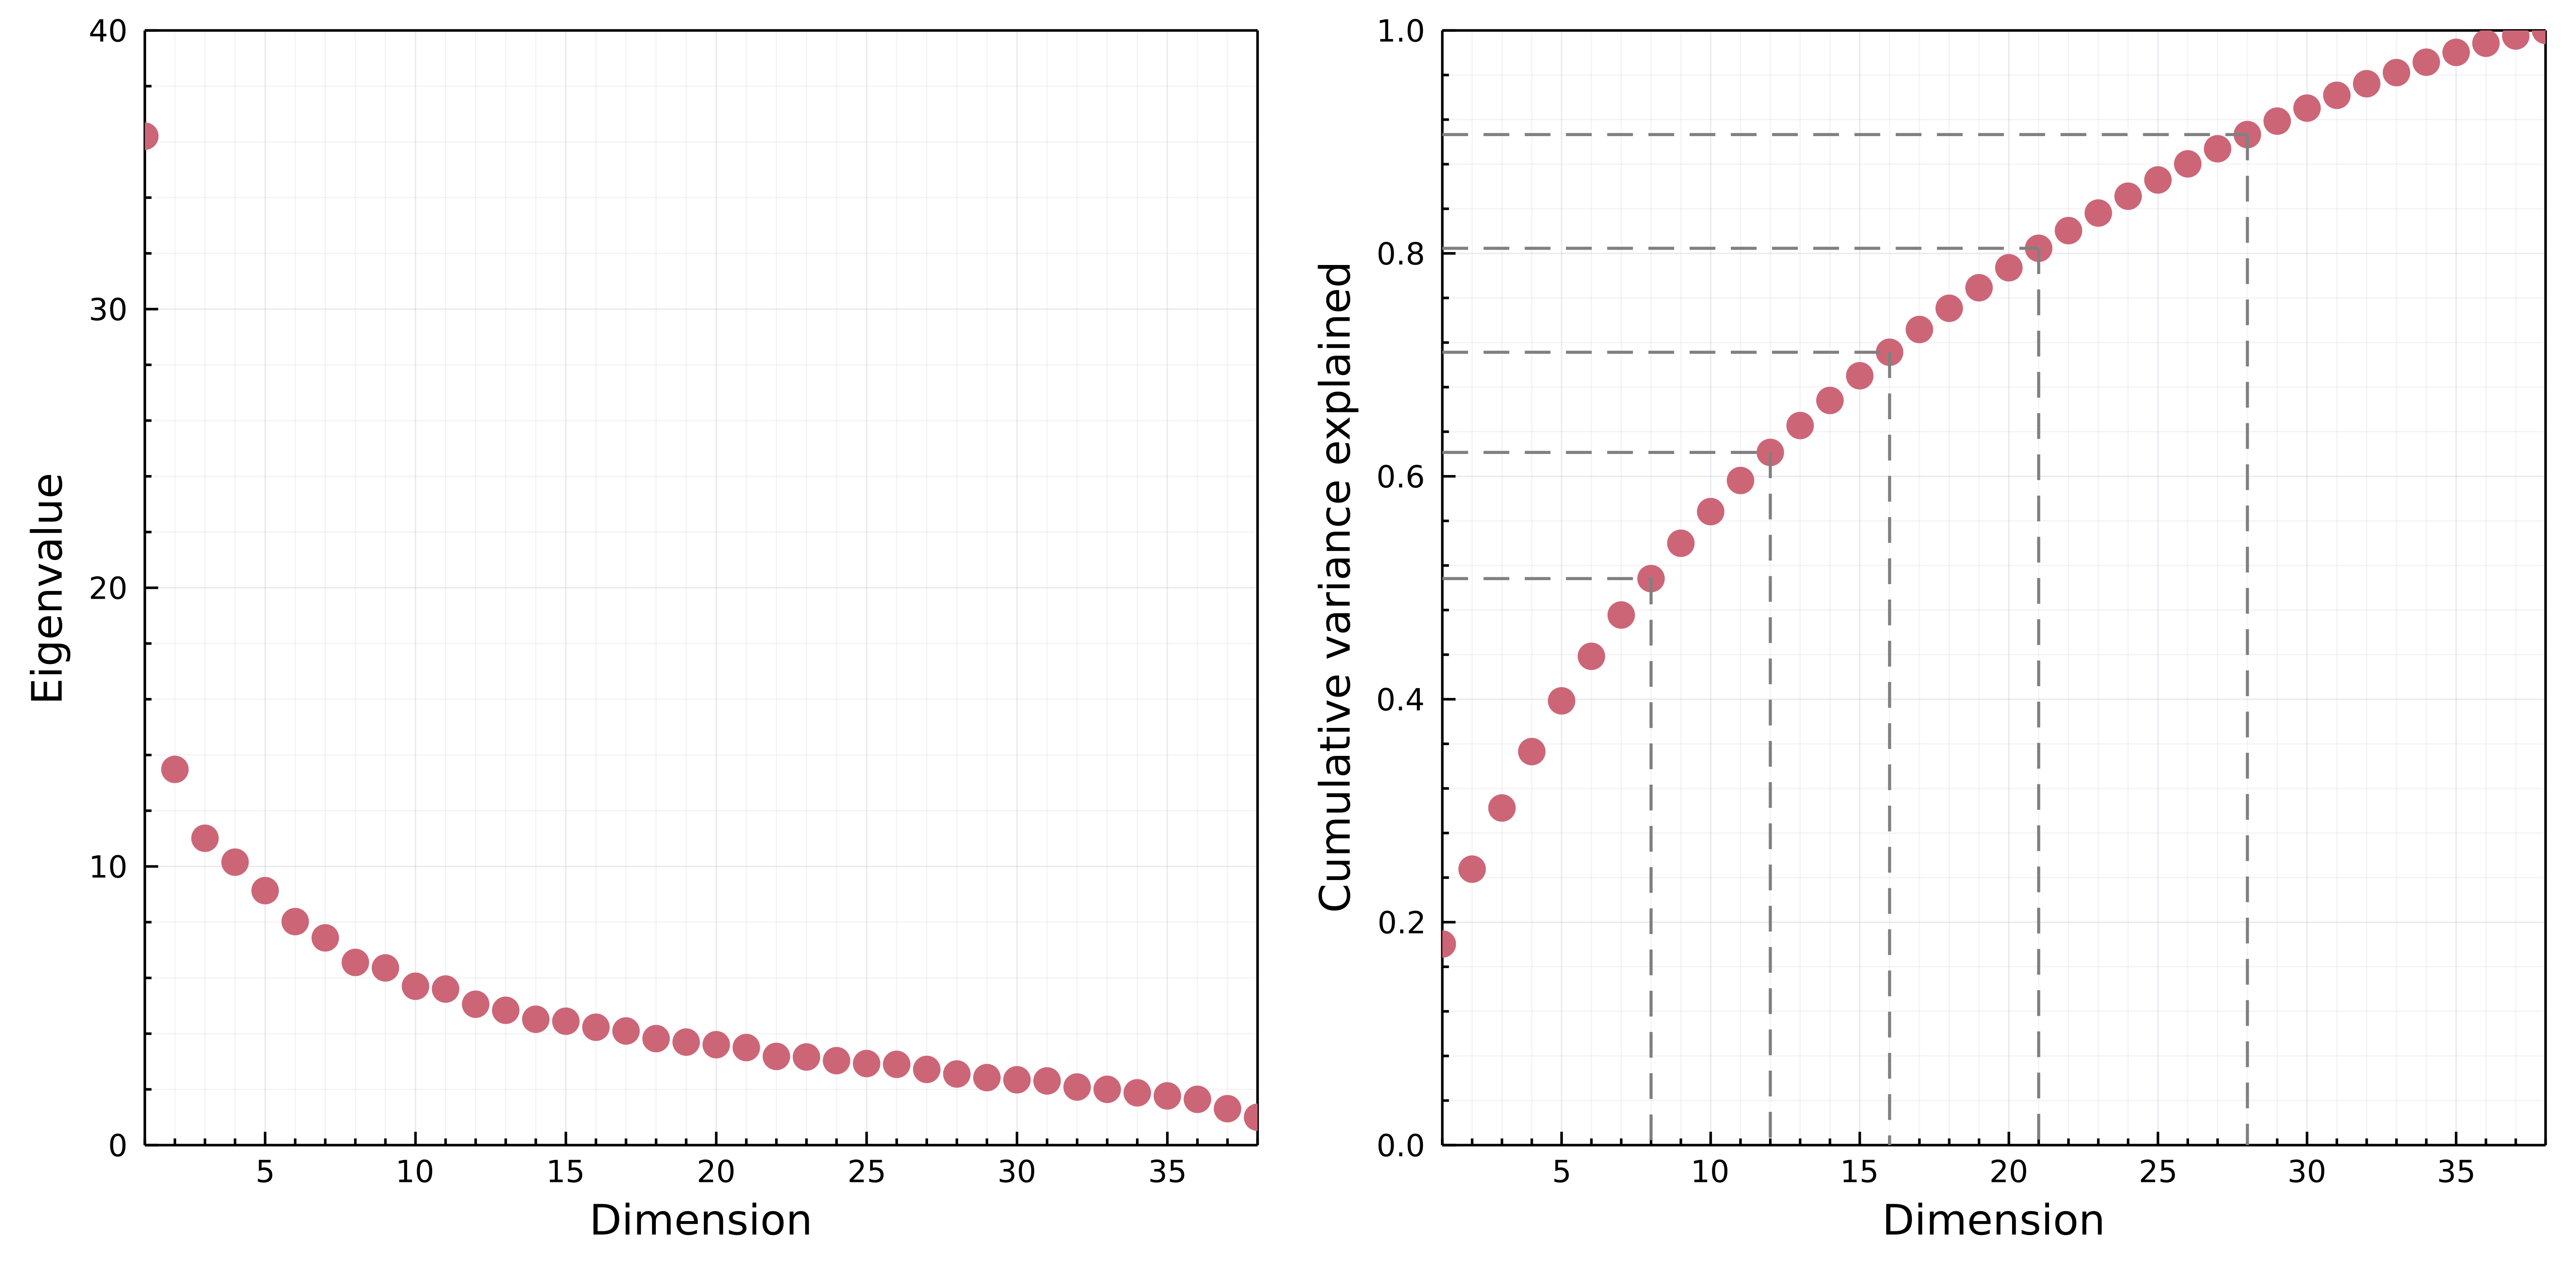
\includegraphics{figures/figure-screeplot.png}
\caption{Left: representation of the screeplot of the singular values
from the t-SVD on the European metaweb. The screeplot shows no obvious
drop in the singular values that may be leveraged to automatically
detect a minimal dimension for embedding, after \emph{e.g.} Zhu and
Ghodsi (2006). Right: cumulative fraction of variance explained by each
dimension up to the rank of the European metaweb. The grey lines
represent cutoffs at 50, 60\ldots{} 90\% of variance explained. For the
rest of the analysis, we reverted to an arbitrary threshold of 60\% of
variance explained, which represented a good tradeoff between accuracy
and reduced number of features.}\label{fig:scree}
}
\end{figure}

Because RDPG relies on matrix multiplication, the higher dimensions
essentially serve to make specific interactions converge towards 0 or 1;
therefore, for reasonably low ranks, there is no guarantee that the
values in the reconstructed network will be within the unit range. In
order to determine what constitutes an appropriate threshold for
probability, we performed the RDPG approach on the European metaweb, and
evaluated the probability threshold by treating this as a binary
classification problem, specifically assuming that both 0 and 1 in the
European metaweb are all true. Given the methodological details given in
Maiorano et al. (2020b) and O'Connor et al. (2020), this seems like a
reasonable assumption, although one that does not hold for all metawebs.
We used the thresholding approach presented in Poisot, Ouellet, et al.
(2021), and picked a cutoff that maximized Youden's \(J\) statistic
(Youden (1950); a measure of the informedness (trust) of predictions);
the resulting cutoff was 0.22, and gave an accuracy above 0.99.

The left and right subspaces for the European metaweb, accompanied by
the threshold for prediction, represent the knowledge we seek to
transfer. In the next section, we explain how we rely on phylogenetic
similarity to do so.

\hypertarget{steps-2-and-3-transfer-learning-through-phylogenetic-relatedness}{%
\subsection{Steps 2 and 3: Transfer learning through phylogenetic
relatedness}\label{steps-2-and-3-transfer-learning-through-phylogenetic-relatedness}}

In order to transfer the knowledge from the European metaweb to the
Canadian species pool, we performed ancestral character estimation using
a Brownian motion model, which is a conservative approach in the absence
of strong hypotheses about the nature of phylogenetic signal in the
network decomposition (Litsios and Salamin 2012). This uses the
estimated feature vectors for the European mammals to create a state
reconstruction for all species (conceptually something akin to a
trait-based mammalian phylogeny using generality and vulnerability
traits) and allows us to impute the missing (latent) trait data for the
Canadian species that are not already in the European network; as we are
focused on predicting contemporary interactions, we only retained the
values for the tips of the three. We assumed that all traits
(\emph{i.e.} the feature vectors for the left and right subspaces) were
independent, which is a reasonable assumption as every trait/dimension
added to the t-SVD has an \emph{additive} effect to the one before it.
Note that the Upham, Esselstyn, and Jetz (2019) tree itself has some
uncertainty associated to inner nodes of the phylogeny. In this case
study, we have decided to not propagate this uncertainty, as it would
complexify the process. The Brownian motion algorithm returns the
\emph{average} value of the trait, and its upper and lower bounds.
Because we do not estimate other parameters of the traits'
distributions, we considered that every species trait is represented as
a uniform distribution between these bounds; in a situation where the
algorithm would return point values for all simulations, one could in
theory either estimate the parameters of a distribution for each tip, or
draw randomly from the outputs. In all cases, the inferred left and
right sub-spaces for the Canadian species pool (\(\hat{\mathcal{L}}\)
and \(\hat{\mathcal{R}}\)) have entries that are distributions,
representing the range of values for a given species at a given
dimension.

These objects represent the transferred knowledge, which we can use for
prediction of the Canadian metaweb.

\hypertarget{step-4-probabilistic-prediction-of-the-destination-network}{%
\subsection{Step 4: Probabilistic prediction of the destination
network}\label{step-4-probabilistic-prediction-of-the-destination-network}}

The phylogenetic reconstruction of \(\hat{\mathcal{L}}\) and
\(\hat{\mathcal{R}}\) has an associated uncertainty, represented by the
breadth of the uniform distribution associated to each of their entries.
Therefore, we can use this information to assemble a
\emph{probabilistic} metaweb in the sense of Poisot et al. (2016),
\emph{i.e.} in which every interaction is represented as a single,
independent, Bernoulli event of probability \(p\).

\begin{figure}
\hypertarget{fig:subspaces}{%
\centering
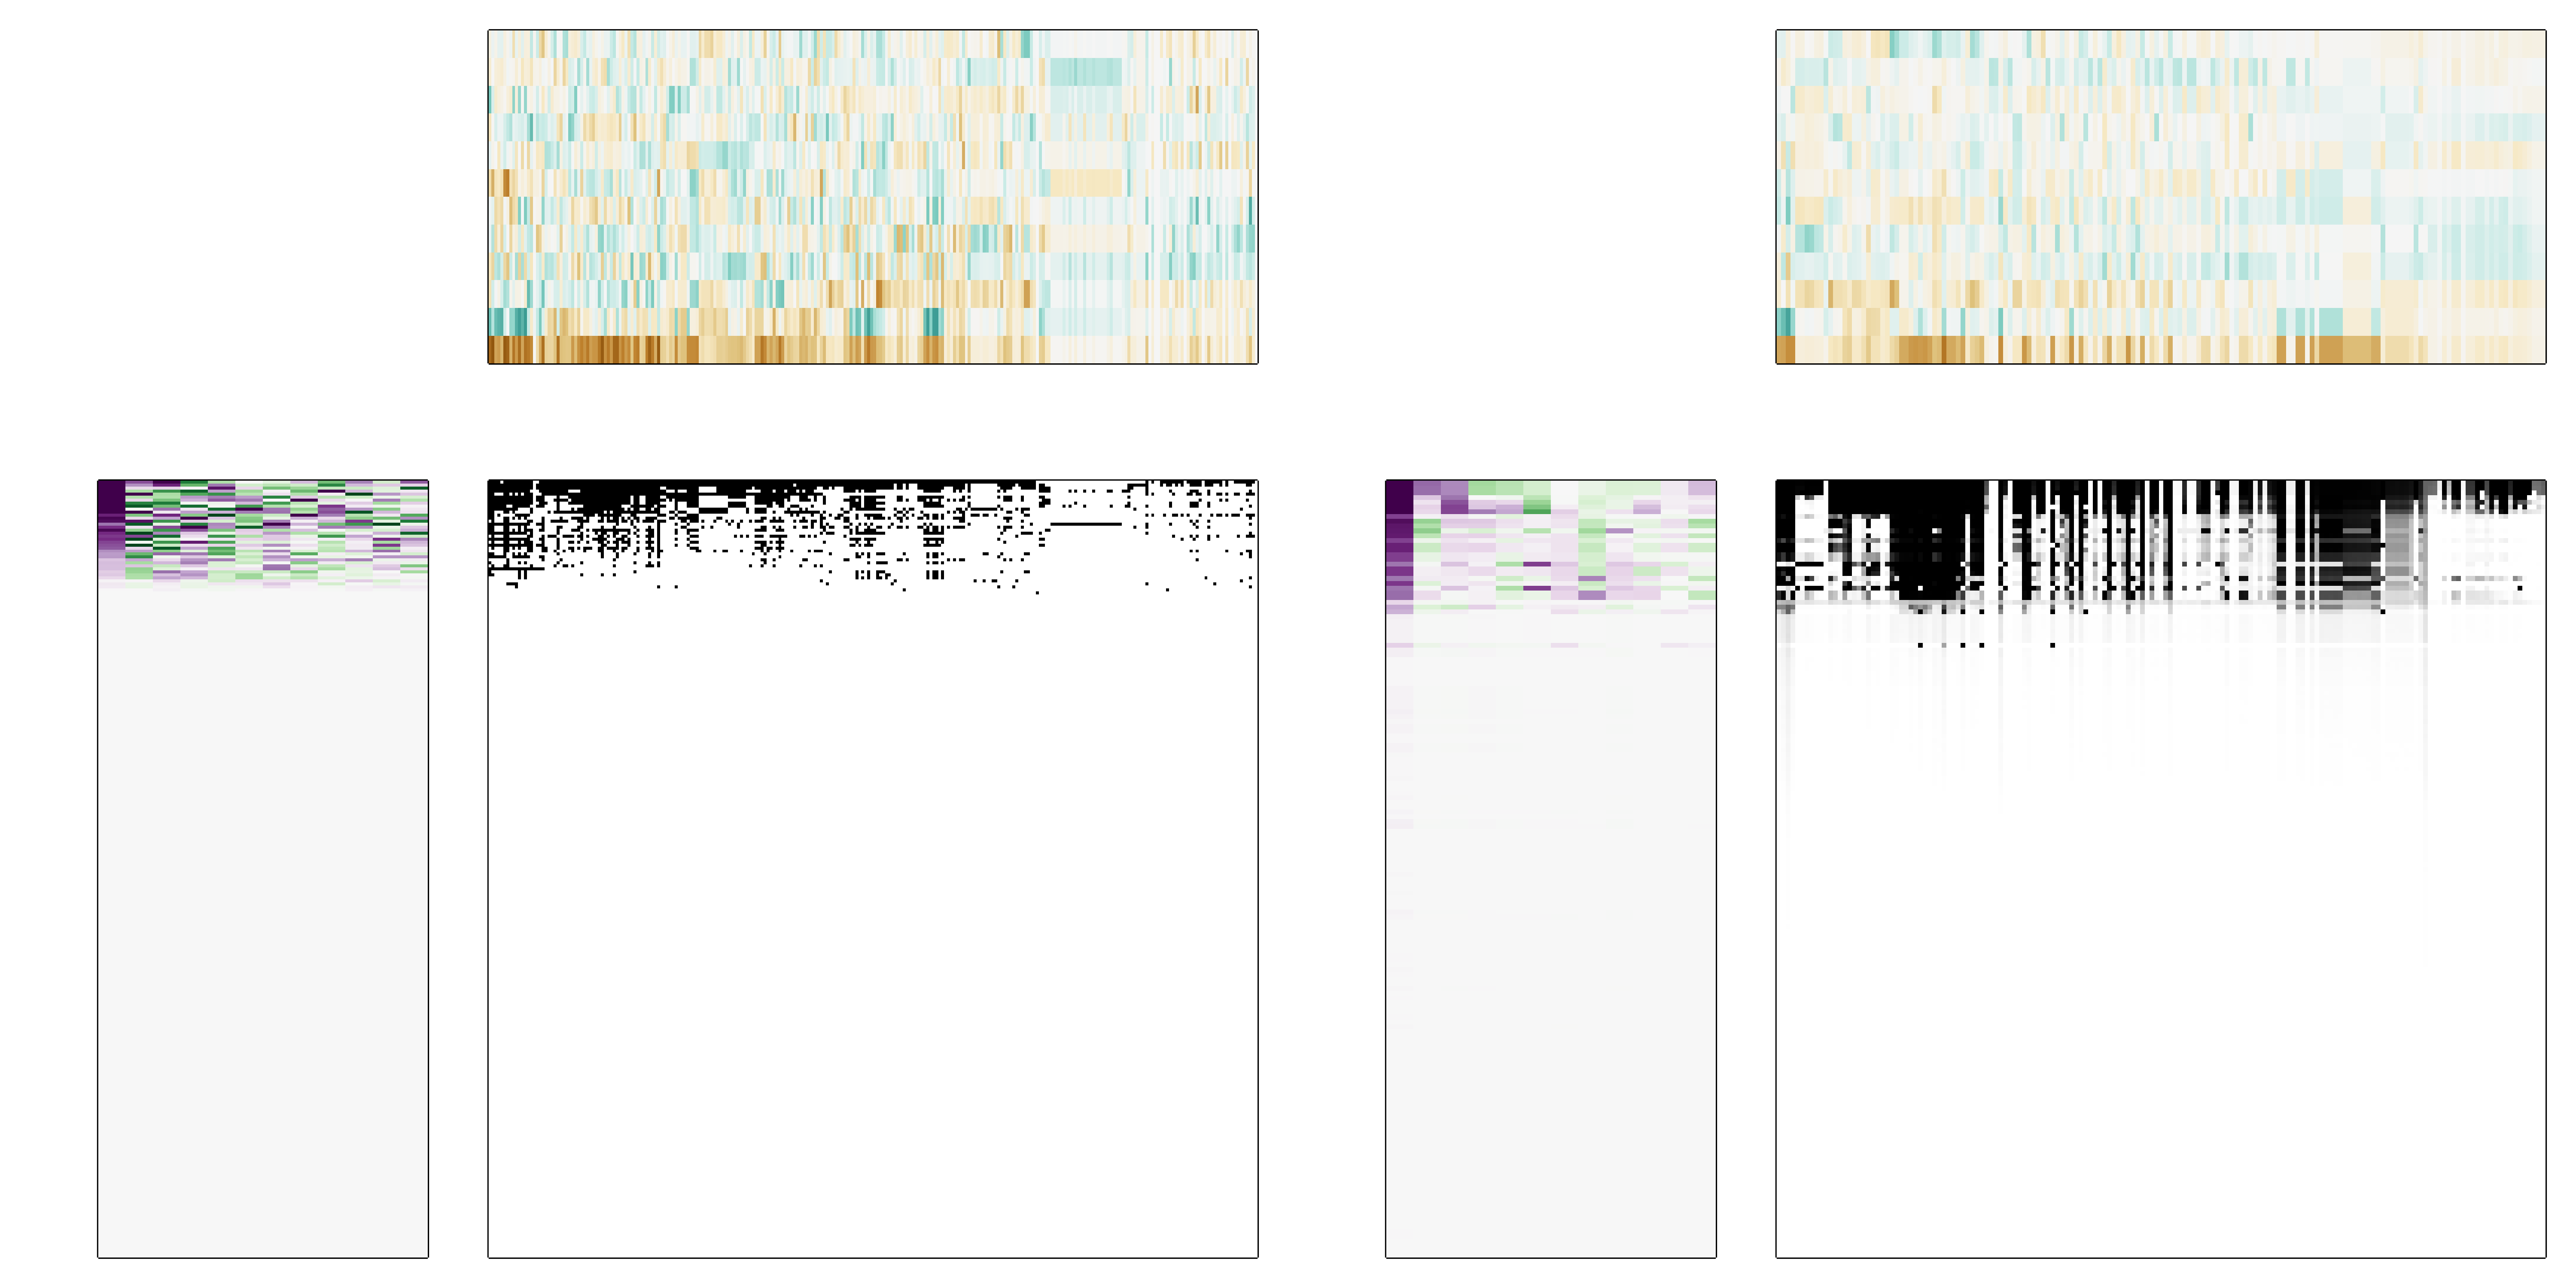
\includegraphics{figures/figure-subspaces.png}
\caption{Visual representation of the left (green/purple) and right
(green/brown) subspaces, alongside the adjacency matrix of the food web
they encode (greyscale). The European metaweb is on the left, and the
imputed Canadian metaweb (before data inflation) on the right. This
figure illustrates how much structure the left sub-space captures. As we
show in fig.~\ref{fig:degree}, the species with a value of 0 in the left
subspace are species without any prey.}\label{fig:subspaces}
}
\end{figure}

Specifically, we have adopted the following approach. For every entry in
\(\hat{\mathcal{L}}\) and \(\hat{\mathcal{R}}\), we draw a value from
its distribution. This results in one instance of the possible left
(\(\hat{\mathcal{l}}\)) and right (\(\hat{\mathcal{r}}\)) subspaces for
the Canadian metaweb. These can be multiplied, to produce one matrix of
real values. Because the entries in \(\hat{\mathcal{l}}\) and
\(\hat{\mathcal{r}}\) are in the same space where \(\mathcal{L}\) and
\(\mathcal{R}\) were originally predicted, it follows that the threshold
\(\rho\) estimated for the European metaweb also applies. We use this
information to produce one random Canadian metaweb,
\(N = \hat{\mathcal{L}}\)\(\hat{\mathcal{R}}' \ge \rho\). As we can see
in (fig.~\ref{fig:subspaces}) the European and Canadian metawebs are
structurally similar (as would be expected given the biogeographic
similarities) and that the two (left and right) subspaces are distinct
\emph{i.e.} capturing predation (generality) and prey (vulnerability)
traits.

Because the intervals around some trait values can be broad (in fact,
probably broader than what they would actually be, see \emph{e.g.}
Garland, Midford, and Ives 1999), we repeat the above process
\(2\times 10^5\) times, which results in a probabilistic metaweb \(P\),
where the probability of an interaction (here conveying our degree of
trust that it exists given the inferred trait distributions) is given by
the number of times where it appears across all random draws \(N\),
divided by the number of samples. An interaction with \(P_{i,j} = 1\)
means that these two species were predicted to interact in all
\(2\times 10^5\) random draws, etc..

\hypertarget{data-cleanup-discovery-validation-and-thresholding}{%
\subsection{Data cleanup, discovery, validation, and
thresholding}\label{data-cleanup-discovery-validation-and-thresholding}}

Once the probabilistic metaweb for Canada has been produced, we followed
a number of data inflation steps to finalize it.

\begin{figure}
\hypertarget{fig:inflation}{%
\centering
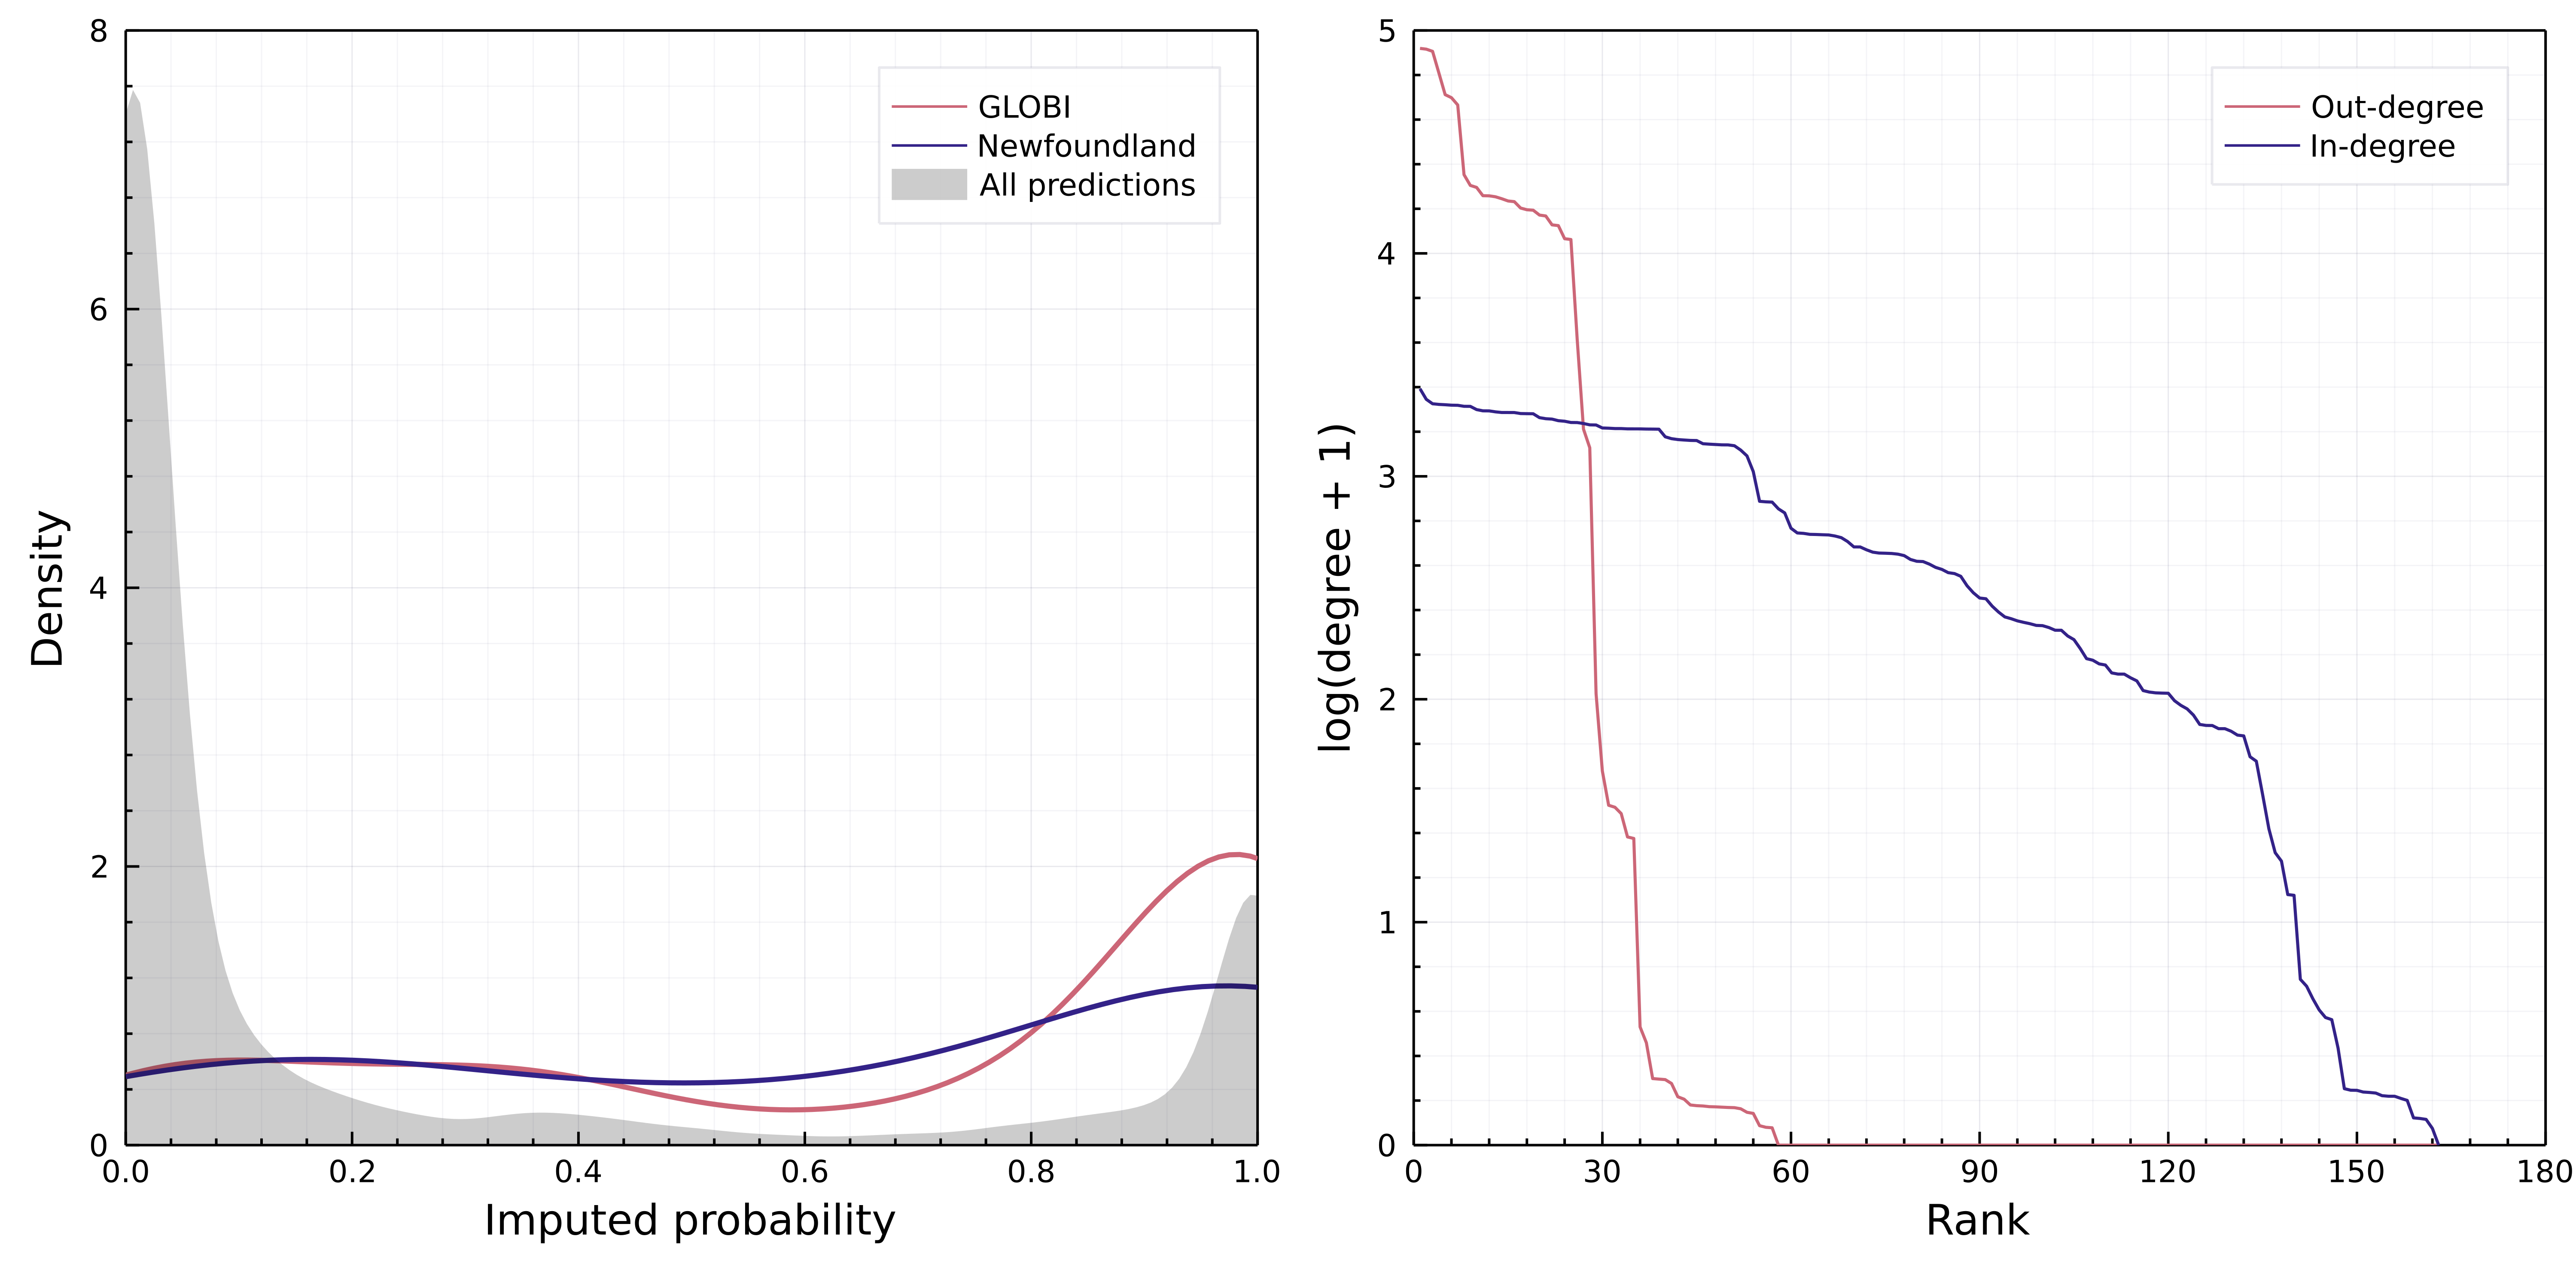
\includegraphics{figures/figure-validation.png}
\caption{Left, comparison of the probabilities of interactions assigned
by the model to all interactions (grey curve), the subset of
interactions found in GLOBI (red), and in the Strong and Leroux (2014)
Newfoundland dataset (blue). The model recovers more interaction with a
low probability compared to data mining, which can suggest that
collected datasets are biased towards more common or easy to identify
interactions. Right, distribution of the in-degree and out-degree of the
mammals from Canada in the reconstructed metaweb. This figure describes
a flat, relatively short food web, in which there are few predators but
a large number of preys.}\label{fig:inflation}
}
\end{figure}

First, we extracted the subgraph corresponding to the 17 species shared
between the European and Canadian pools and replaced these interactions
with a probability of 0 (non-interaction) or 1 (interaction). This
represents a minute modification of the inferred network (about 0.8\% of
all species pairs from the Canadian web), but ensures that we are
directly re-using knowledge from Europe.

Second, we looked for all species in the Canadian pool known to the
Global Biotic Interactions (GLoBI) database (Poelen, Simons, and Mungall
2014), and extracted their known interactions. Because GLOBI aggregates
observed interactions, it is not a \emph{networks} data source, and
therefore the only information we can reliably extract from it is that a
species pair \emph{was reported to interact at least once}. This last
statement should yet be taken with caution, as some sources in GLOBI
(\emph{e.g.} Thessen and Parr 2014) are produced though text analysis,
and therefore may not document direct evidence of the interaction.
Nevertheless, should the predictive model work, we would expect that a
majority of interactions known to GLOBI would also be predicted. After
performing this check, we set the probability of all interactions known
to GLOBI (366 in total, 33 of which were not predicted by the model, for
a success rate of 91\%) to 1.

Finally, we downloaded the data from Strong and Leroux (2014), who mined
various literature sources to identify trophic interactions in
Newfoundland. This dataset documented 25 interactions between mammals,
only two of which were not part of our (Canada-level) predictions,
resulting in a success rate of 92\%. These two interactions were added
to our predicted metaweb with a probability of 1.

\begin{figure}
\hypertarget{fig:thresholds}{%
\centering
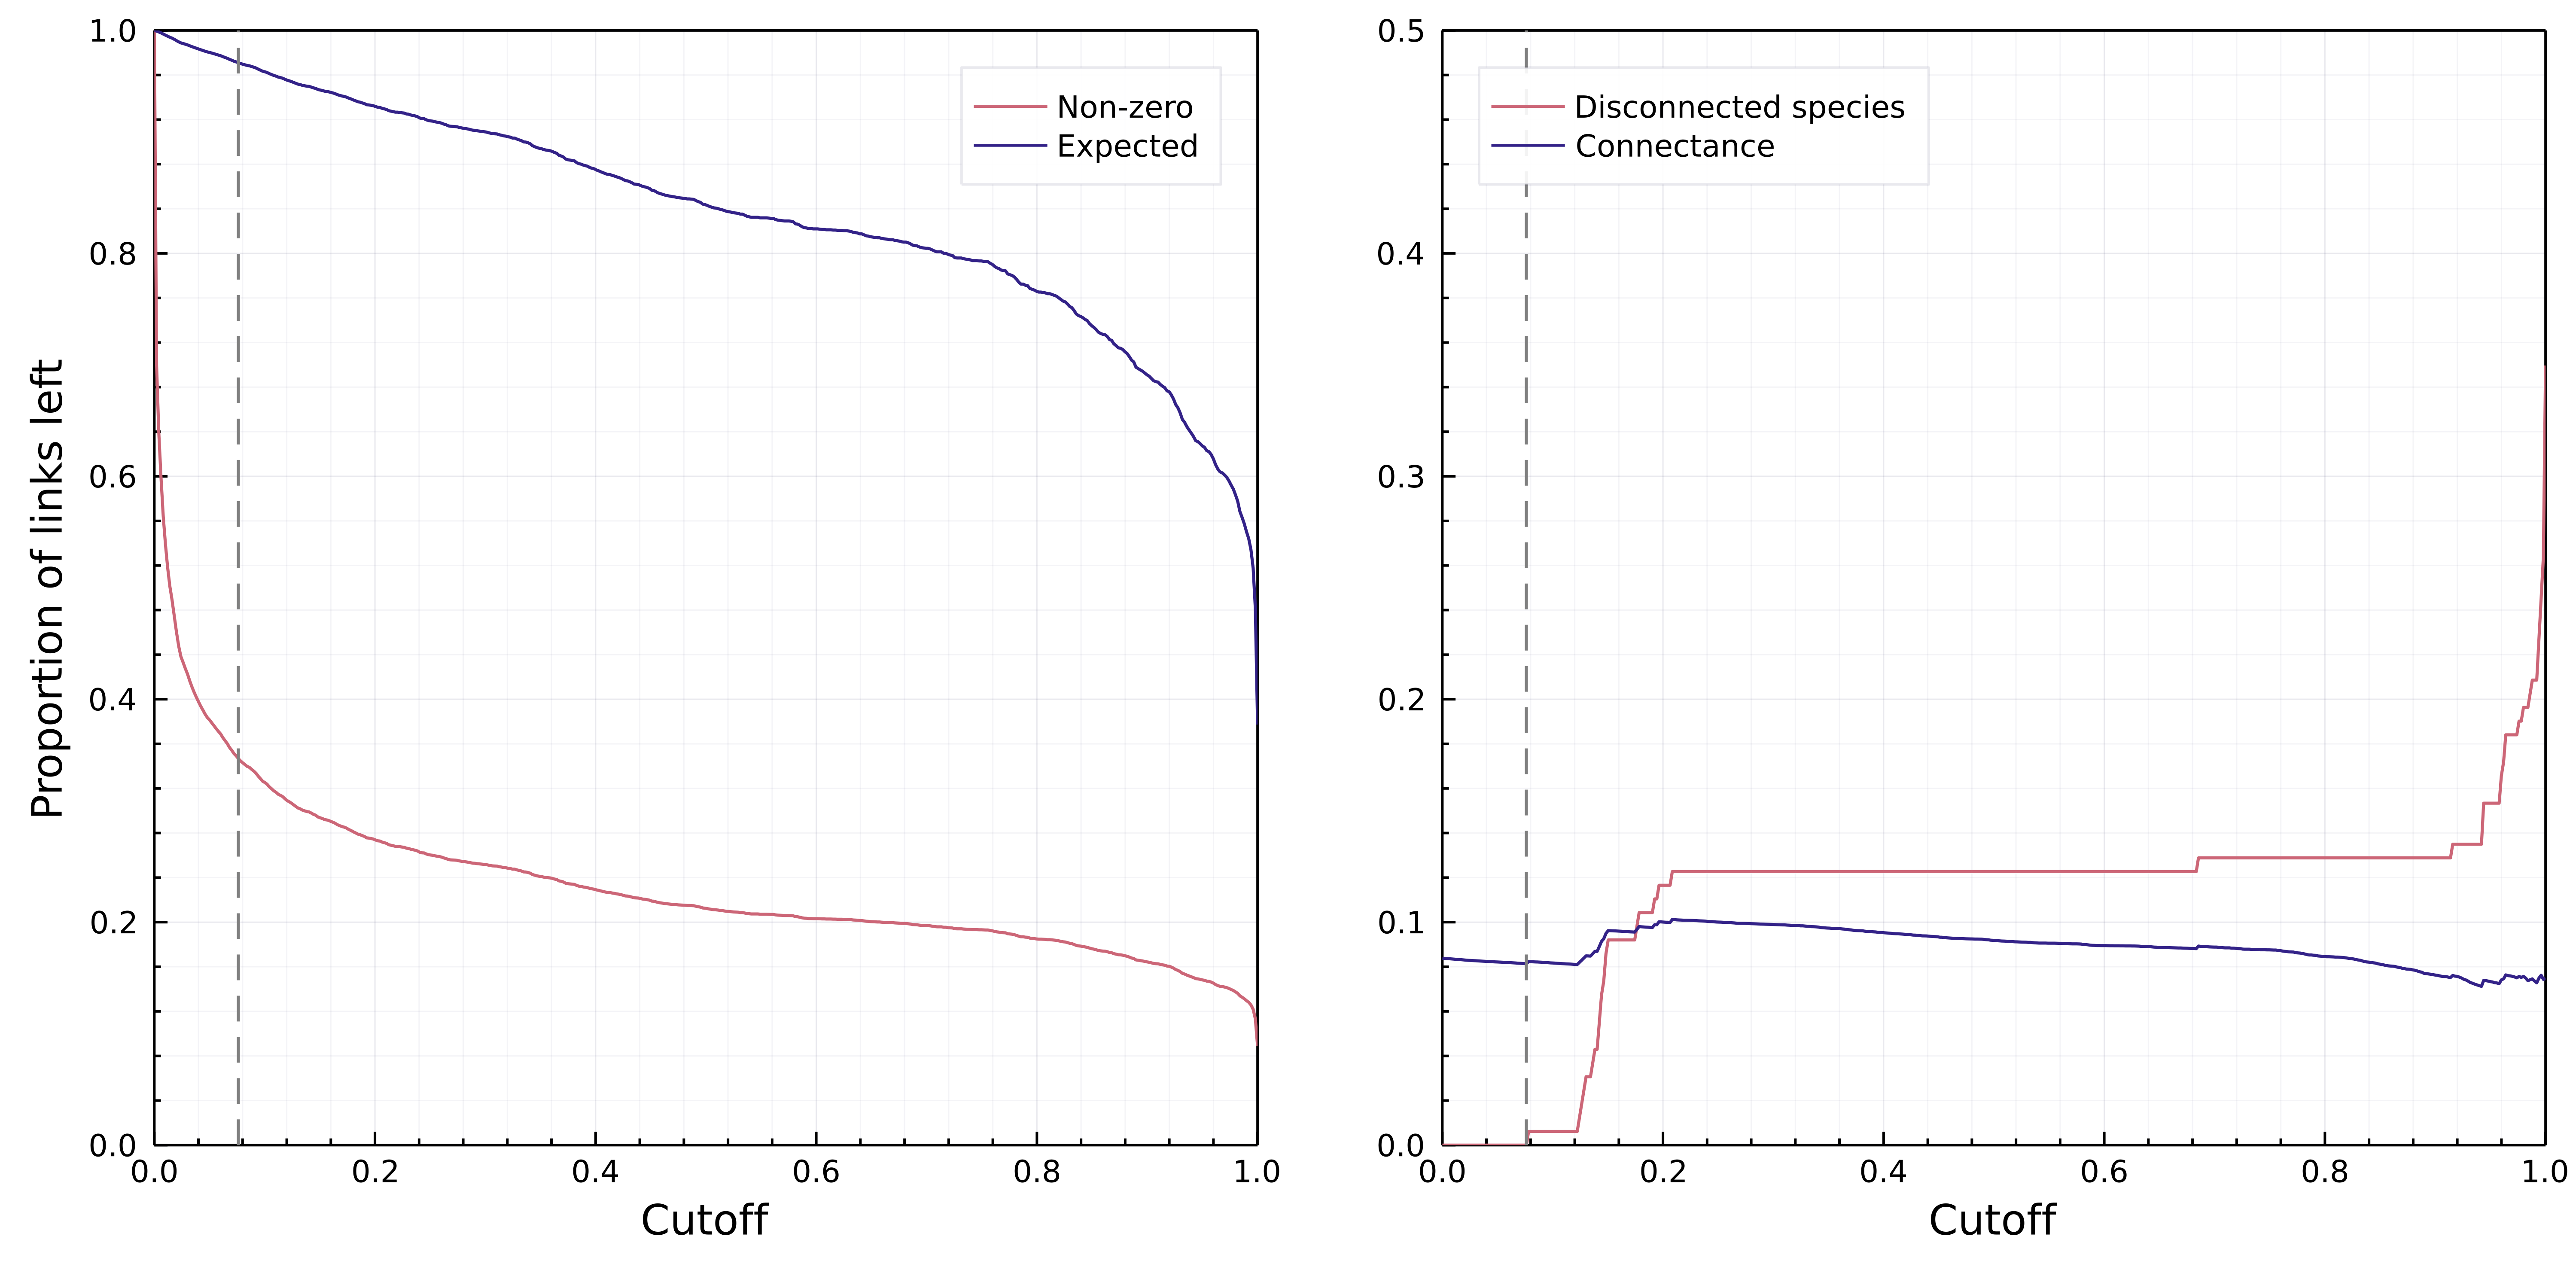
\includegraphics{figures/figure-cutoffs.png}
\caption{Left: effect of varying the cutoff for probabilities to be
considered non-zero on the number of unique links and on \(\hat{L}\),
the probabilistic estimate of the number of links assuming that all
interactions are independent. Right: effect of varying the cutoff on the
number of disconnected species, and on network connectance. In both
panels, the grey line indicates the cutoff
\(P(i\rightarrow j) \approx 0.08\) that resulted in the first species
losing all of its interactions.}\label{fig:thresholds}
}
\end{figure}

Because the confidence intervals on the inferred trait space are
probably over-estimates, we decided to apply a thresholding step to the
interactions after the data inflation (fig.~\ref{fig:thresholds}).
Cirtwill and Hambäck (2021) proposed a number of strategies to threshold
probabilistic networks. Their methods assume the underlying data to be
tag-based sequencing, which represents interactions as co-occurrences of
predator and prey within the same tags; this is conceptually identical
to our Bernoulli-trial based reconstruction of a probabilistic network.
We performed a full analysis of the effect of various cutoffs, and as
they either resulted in removing too few interactions, or removing
enough interactions that species started to be disconnected from the
network, we set this threshold for a probability equivalent to 0 to the
largest possible value that still allowed all species to have at least
one interaction with a non-zero probability. The need for this slight
deviation from the Cirtwill and Hambäck (2021) method highlights the
need for additional development on network thresholding.

\hypertarget{results-and-discussion-of-the-case-study}{%
\section{Results and discussion of the case
study}\label{results-and-discussion-of-the-case-study}}

In fig.~\ref{fig:thresholds}, we examine the effect of varying the
cutoff on \(P(i \rightarrow j)\) on the number of links, species, and
connectance. Determining a cutoff using the maximum curvature, or
central difference approximation of the second order partial derivative,
as suggested by \emph{e.g.} Cirtwill and Hambäck (2021), results in
respectively species being lost, or almost all links being kept. We
therefore settled on the value that allowed all species to remain with
at least one interaction. This result, in and of itself, suggests that
additional methodological developments for the thresholding of
probabilistic networks are required.

\begin{figure}
\hypertarget{fig:degree}{%
\centering
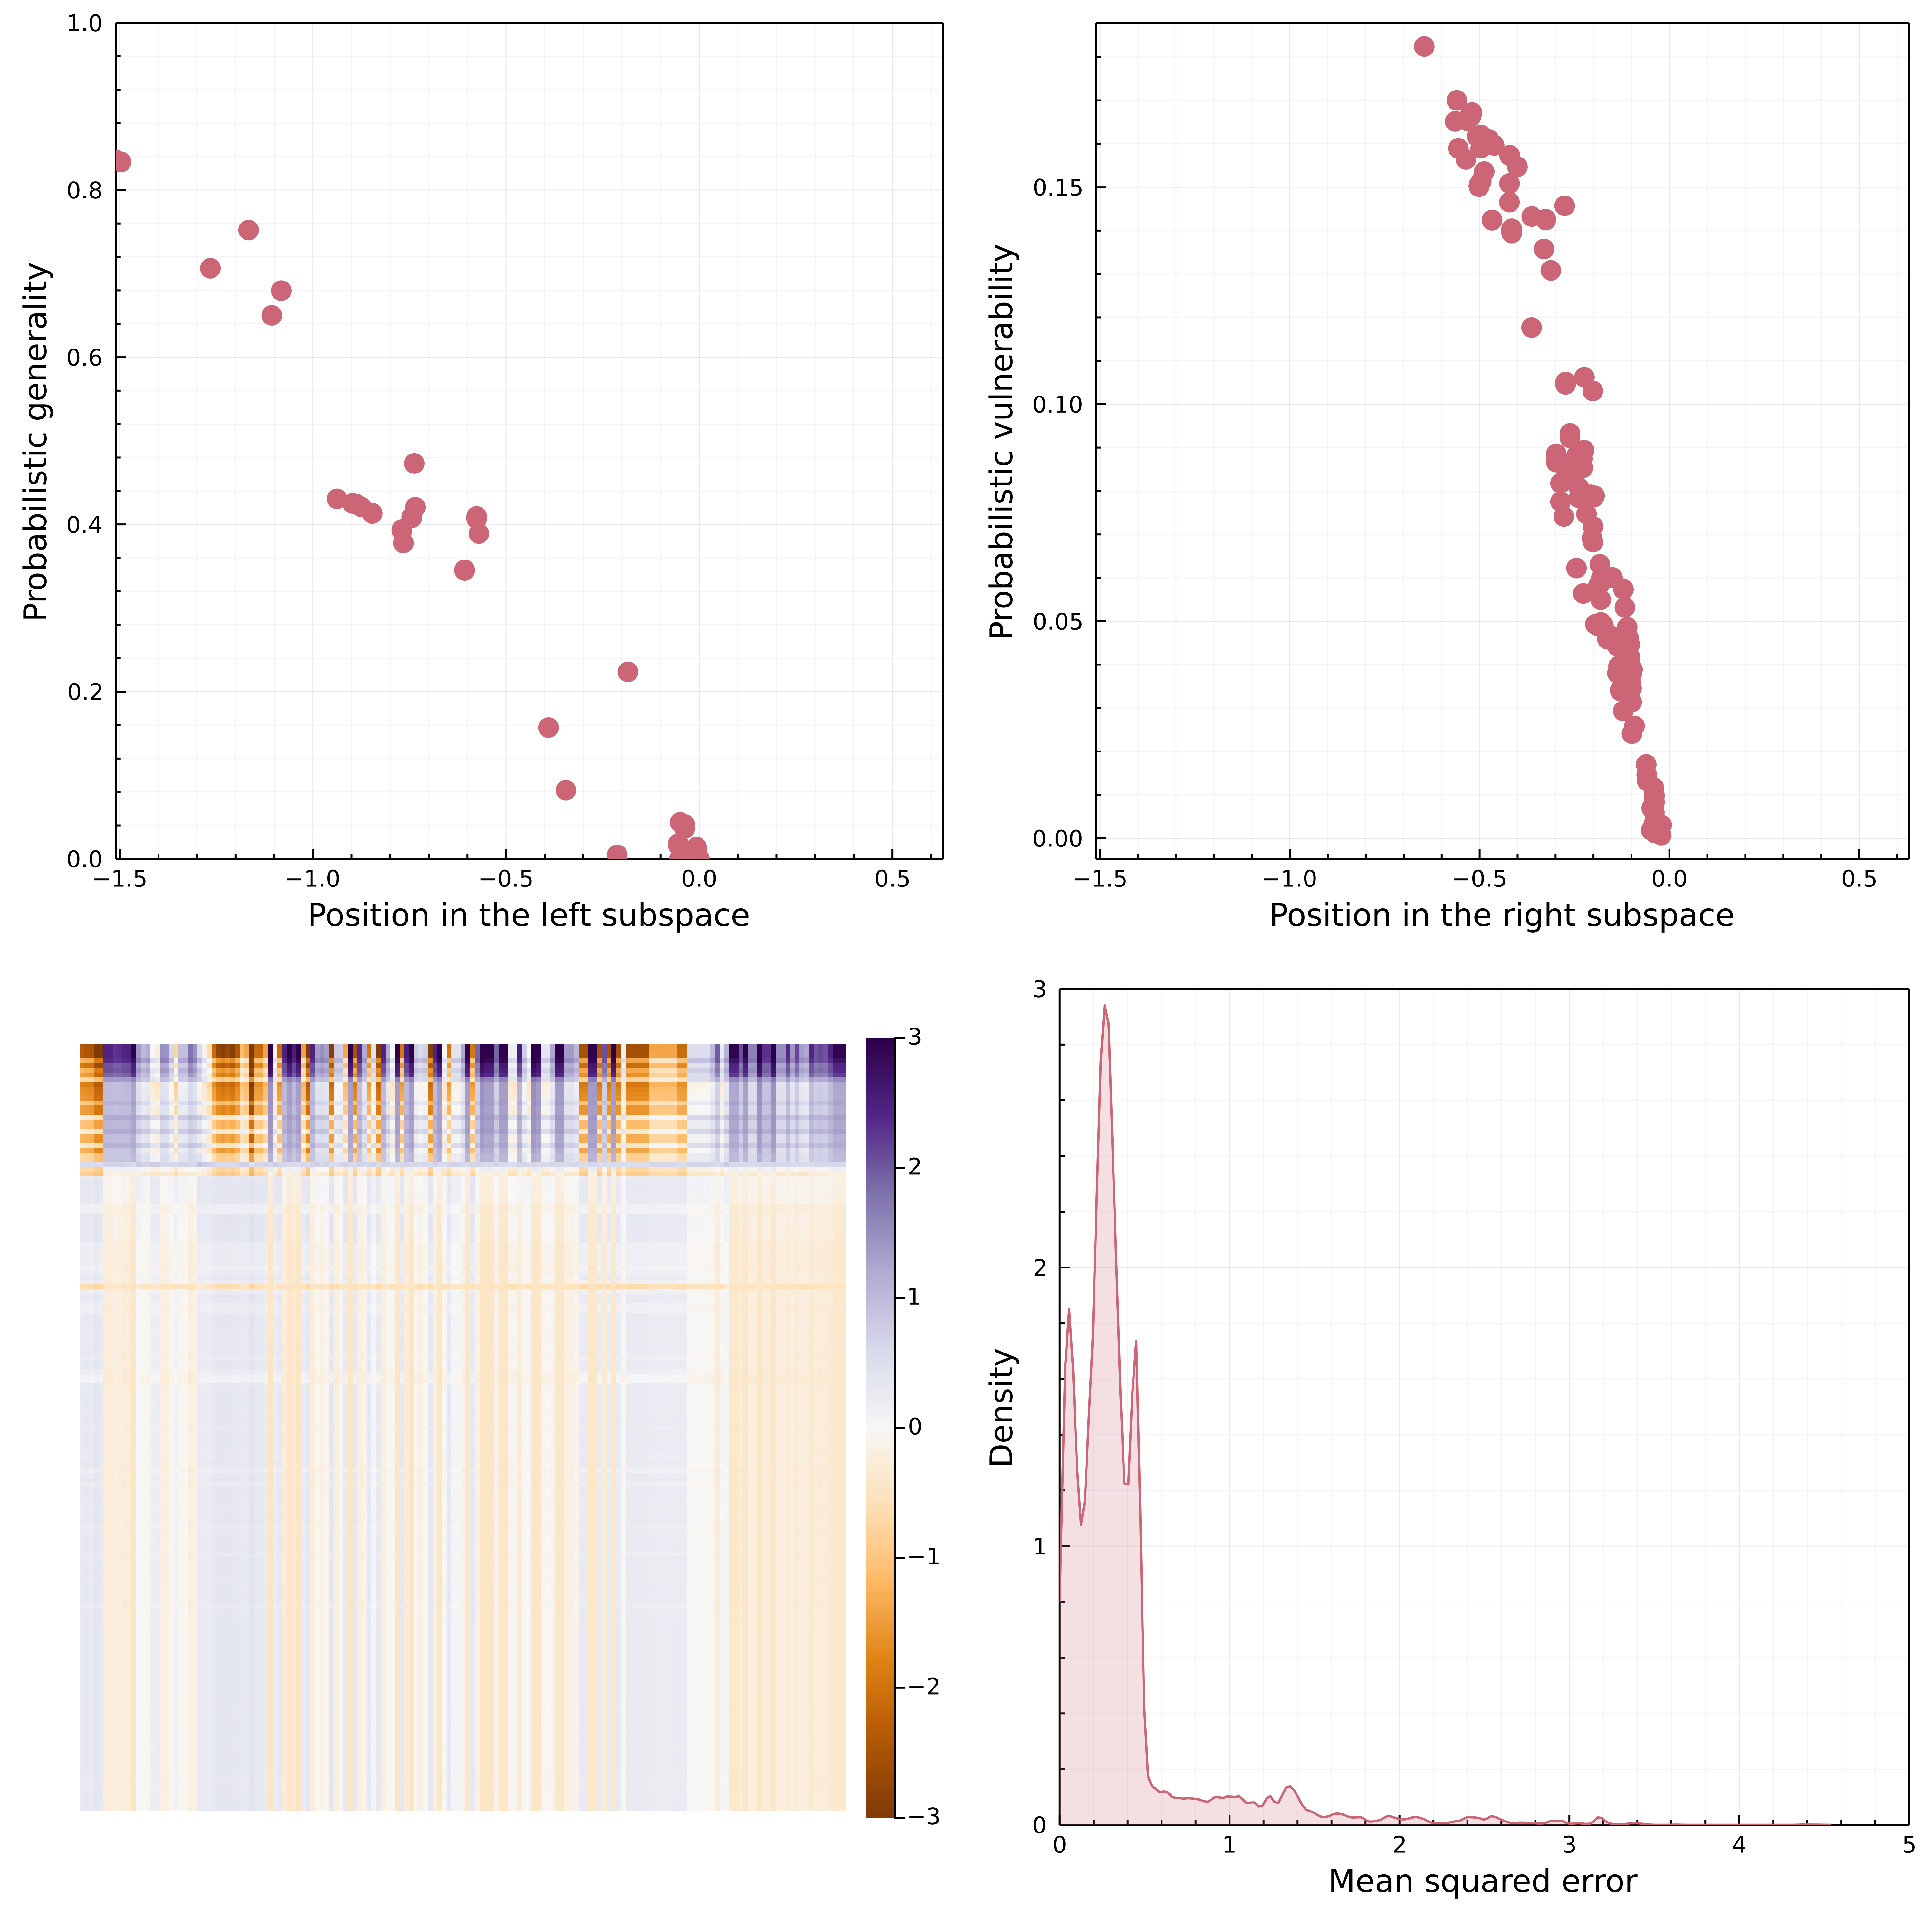
\includegraphics{figures/figure-degree.png}
\caption{Top: biological significance of the first dimension. Left:
there is a linear relationship between the values on the first dimension
of the left subspace and the generality, \emph{i.e.} the relative number
of preys, \emph{sensu} Schoener (1989). Species with a value of 0 in
this subspace are at the bottom-most trophic level. Right: there is,
similarly, a linear relationship between the position of a species on
the first dimension of the right subspace and its vulnerability,
\emph{i.e.} the relative number of predators. Taken together, these two
figures show that the first-order representation of this network would
capture its degree distribution. Bottom: topological consequences of the
first dimension. Left: differences in the \(z\)-score of the actual
configuration model for the reconstructed network, and the prediction
based only on the first dimension. Right: distribution of the
differences in the left panel.}\label{fig:degree}
}
\end{figure}

The t-SVD embedding is able to learn relevant ecological features for
the network. fig.~\ref{fig:degree} shows that the first rank correlates
linearly with generality and vulnerability (Schoener 1989), \emph{i.e.}
the number of preys and predators. Importantly, this implies that a rank
1 approximation represents the configuration model for the metaweb,
\emph{i.e.} a set of random networks generated from a given degree
sequence (Park and Newman 2004). Accounting for the probabilistic nature
of the degrees, the rank 1 approximation also represents the \emph{soft}
configuration model (van der Hoorn, Lippner, and Krioukov 2018). Both
models are maximum entropy graph models (Garlaschelli, Hollander, and
Roccaverde 2018), with sharp (all network realizations satisfy the
specified degree sequence) and soft (network realizations satisfy the
degree sequence on average) local constraints, respectively. The (soft)
configuration model is an unbiased random graph model widely used by
ecologists in the context of null hypothesis significance testing of
network structure (\emph{e.g.} Bascompte et al. 2003) and can provide
informative priors for Bayesian inference of network structure
(\emph{e.g.} J.-G. Young, Cantwell, and Newman 2021). It is noteworthy
that for this metaweb, the relevant information was extracted at the
first rank. Because the first rank corresponds to the leading singular
value of the system, the results of fig.~\ref{fig:degree} have a
straightforward interpretation: degree-based processes are the most
important in structuring the mammalian food web.

\hypertarget{discussion}{%
\section{Discussion}\label{discussion}}

One important aspect in which Europe and Canada differ (despite their
comparable bioclimatic conditions) is the legacy of human impacts, which
have been much longer in Europe. Nenzén, Montoya, and Varela (2014)
showed that even at small scales (the Iberian peninsula), mammal food
webs retain the signal of both climate change and human activity, even
when this human activity was orders of magnitude less important than it
is now. Similarly, Yeakel et al. (2014) showed that changes in human
occupation over several centuries can lead to food web collapse.
Megafauna in particular seems to be very sensitive to human arrival
(Pires et al. 2015). In short, there is well-substantiated support for
the idea that human footprint affects more than the risk of species
extinction (Marco et al. 2018), and can lead to changes in interaction
structure. Yet, owing to the inherent plasticity of interactions, there
have been documented instances of food webs undergoing rapid
collapse/recovery cycles over short periods of time (Pedersen et al.
2017). The embedding of a network, in a sense, embeds its
macro-evolutionary history, especially as RDPG captures ecological
signal (Dalla Riva and Stouffer 2016); at this point, it is important to
recall that a metaweb is intended as a catalogue of all possible
interactions, which should then be filtered (Morales-Castilla et al.
2015). In practice (and in this instance) the reconstructed metaweb will
predict interactions that are plausible based on the species'
evolutionary history, however some interactions would not be realized
due to human impact.

Cirtwill et al. (2019) previously made the point that network inference
techniques based on Bayesian approaches would perform far better in the
presence of an interaction-level informative prior; the desirable
properties of such a prior would be that it is expressed as a
probability, preferably representing a Bernoulli event, the value of
which would be representative of relevant biological processes. We argue
that the probability returned at the very last step of our framework may
serve as this informative prior; indeed, the output of our analysis can
be used in subsequent steps, also possibly involving expert elicitation
to validate some of the most strongly recommended interactions. One
important \emph{caveat} to keep in mind when working with interaction
inference is that interactions can never really be true negatives (in
the current state of our methodological framework and data collection
limitations); this renders the task of validating a model through the
usual application of binary classification statistics very difficult
(although see Strydom et al. 2021 for a discussion of alternative
suggestions).

As Herbert (1965) rightfully pointed out, ``{[}y{]}ou can't draw neat
lines around planet-wide problems''; in this regard, our approach must
contend with two interesting problems. The first is the limit of the
metaweb to embed and transfer. If the initial metaweb is too narrow in
scope, notably from a taxonomic point of view, the chances of finding
another area with enough related species to make a reliable inference
decrease. This is notably true if the metaweb is assembled in an area
with mostly endemic species. Conversely, the metaweb should be reliably
filled, which assumes that the \(S^2\) interactions in a pool of \(S\)
species have been examined, either through literature surveys or expert
elicitation. The second problem is to determine which area should be
used to infer the new metaweb in, as this determines the species pool
that must be used. In our application, we focused on the mammals of
Canada. The upside of this approach is that information at the country
level is likely to be required by policy makers and stakeholders for
their biodiversity assessment, as each country tends to set goals at the
national level (Buxton et al. 2021) for which quantitative instruments
are designed (Turak et al. 2017), with specific strategies often enacted
at smaller scales (Ray, Grimm, and Olive 2021). Yet these national
divisions, in large parts of the world, reflect nothing except for the
legacy of settler colonialism, and operating under them must be done
under the clear realization that they contributed to the ongoing
biodiversity crisis (Adam 2014), can reinforce environmental injustice
(Choudry 2013; Domínguez and Luoma 2020), and on Turtle Island
especially, will probably end up being replaced by Indigenous principles
of land management (Eichhorn, Baker, and Griffiths 2019; No'kmaq et al.
2021).

\textbf{Acknowledgements:} We acknowledge that this study was conducted
on land within the traditional unceded territory of the Saint Lawrence
Iroquoian, Anishinabewaki, Mohawk, Huron-Wendat, and Omàmiwininiwak
nations. TP, TS, DC, and LP received funding from the Canadian Institue
for Ecology \& Evolution. FB is funded by the Institut de Valorisation
des Données. TS, SB, and TP are funded by a donation from the Courtois
Foundation. CB was awarded a Mitacs Elevate Fellowship no. IT12391, in
partnership with fRI Research, and also acknowledges funding from
Alberta Innovates and the Forest Resources Improvement Association of
Alberta. M-JF acknowledges funding from NSERC Discovery Grant and NSERC
CRC RR is funded by New Zealand's Biological Heritage Ngā Koiora Tuku
Iho National Science Challenge, administered by New Zealand Ministry of
Business, Innovation, and Employment. BM is funded by the NSERC
Alexander Graham Bell Canada Graduate Scholarship and the FRQNT master's
scholarshipTP acknowledges financial support from NSERC through the
Discovery Grants and Discovery Accelerator Supplement programs.

\hypertarget{references}{%
\section*{References}\label{references}}
\addcontentsline{toc}{section}{References}

\hypertarget{refs}{}
\begin{CSLReferences}{1}{0}
\leavevmode\hypertarget{ref-Adam2014EleTre}{}%
Adam, Rachelle. 2014. \emph{Elephant Treaties: The Colonial Legacy of
the Biodiversity Crisis}. UPNE.

\leavevmode\hypertarget{ref-Albouy2019MarFis}{}%
Albouy, Camille, Philippe Archambault, Ward Appeltans, Miguel B. Araújo,
David Beauchesne, Kevin Cazelles, Alyssa R. Cirtwill, et al. 2019.
{``The Marine Fish Food Web Is Globally Connected.''} \emph{Nature
Ecology \& Evolution} 3 (8): 1153--61.
\url{https://doi.org/10.1038/s41559-019-0950-y}.

\leavevmode\hypertarget{ref-Banville2021ManJl}{}%
Banville, Francis, Steve Vissault, and Timothée Poisot. 2021.
{``Mangal.jl and EcologicalNetworks.jl: Two Complementary Packages for
Analyzing Ecological Networks in Julia.''} \emph{Journal of Open Source
Software} 6 (61): 2721. \url{https://doi.org/10.21105/joss.02721}.

\leavevmode\hypertarget{ref-Bascompte2003NesAss}{}%
Bascompte, J., P. Jordano, C. J. Melian, and J. M. Olesen. 2003. {``The
Nested Assembly of Plant-Animal Mutualistic Networks.''}
\emph{Proceedings of the National Academy of Sciences} 100 (16):
9383--87. \url{https://doi.org/10.1073/pnas.1633576100}.

\leavevmode\hypertarget{ref-Beckerman2006ForBio}{}%
Beckerman, Andrew P., Owen L. Petchey, and Philip H. Warren. 2006.
{``Foraging Biology Predicts Food Web Complexity.''} \emph{Proceedings
of the National Academy of Sciences} 103 (37): 13745--49.
\url{https://doi.org/10.1073/pnas.0603039103}.

\leavevmode\hypertarget{ref-Bezanson2017JulFre}{}%
Bezanson, J., A. Edelman, S. Karpinski, and V. Shah. 2017. {``Julia: A
Fresh Approach to Numerical Computing.''} \emph{SIAM Review} 59 (1):
65--98. \url{https://doi.org/10.1137/141000671}.

\leavevmode\hypertarget{ref-Boeckaerts2021PreBac}{}%
Boeckaerts, Dimitri, Michiel Stock, Bjorn Criel, Hans Gerstmans, Bernard
De Baets, and Yves Briers. 2021. {``Predicting Bacteriophage Hosts Based
on Sequences of Annotated Receptor-Binding Proteins.''} \emph{Scientific
Reports} 11 (1): 1467. \url{https://doi.org/10.1038/s41598-021-81063-4}.

\leavevmode\hypertarget{ref-Braga2021PhyRec}{}%
Braga, Mariana P., Niklas Janz, Sören Nylin, Fredrik Ronquist, and
Michael J. Landis. 2021. {``Phylogenetic Reconstruction of Ancestral
Ecological Networks Through Time for Pierid Butterflies and Their Host
Plants.''} \emph{Ecology Letters} n/a (n/a).
\url{https://doi.org/10.1111/ele.13842}.

\leavevmode\hypertarget{ref-Buxton2021KeyInf}{}%
Buxton, Rachel T., Joseph R. Bennett, Andrea J. Reid, Charles Shulman,
Steven J. Cooke, Charles M. Francis, Elizabeth A. Nyboer, et al. 2021.
{``Key Information Needs to Move from Knowledge to Action for
Biodiversity Conservation in Canada.''} \emph{Biological Conservation}
256: 108983. \url{https://doi.org/10.1016/j.biocon.2021.108983}.

\leavevmode\hypertarget{ref-Cameron2019UneGlo}{}%
Cameron, Erin K., Maja K. Sundqvist, Sally A. Keith, Paul J. CaraDonna,
Erik A. Mousing, Karin A. Nilsson, Daniel B. Metcalfe, and Aimée T.
Classen. 2019. {``Uneven Global Distribution of Food Web Studies Under
Climate Change.''} \emph{Ecosphere} 10 (3): e02645.
\url{https://doi.org/10.1002/ecs2.2645}.

\leavevmode\hypertarget{ref-Cavender-Bares2009MerCom}{}%
Cavender-Bares, Jeannine, Kenneth H. Kozak, Paul V. A. Fine, and Steven
W. Kembel. 2009. {``The Merging of Community Ecology and Phylogenetic
Biology.''} \emph{Ecology Letters} 12 (7): 693--715.
\url{https://doi.org/10.1111/j.1461-0248.2009.01314.x}.

\leavevmode\hypertarget{ref-Choudry2013SavBio}{}%
Choudry, Aziz. 2013. {``Saving Biodiversity, for Whom and for What?
Conservation NGOs, Complicity, Colonialism and Conquest in an Era of
Capitalist Globalization.''} In \emph{NGOization: Complicity,
Contradictions and Prospects}, 24--44. Bloomsbury Publishing.

\leavevmode\hypertarget{ref-Cirtwill2019QuaFra}{}%
Cirtwill, Alyssa R., Anna Eklf, Tomas Roslin, Kate Wootton, and
Dominique Gravel. 2019. {``A Quantitative Framework for Investigating
the Reliability of Empirical Network Construction.''} \emph{Methods in
Ecology and Evolution} 0 (ja).
\url{https://doi.org/10.1111/2041-210X.13180}.

\leavevmode\hypertarget{ref-Cirtwill2021BuiFoo}{}%
Cirtwill, Alyssa R., and Peter Hambäck. 2021. {``Building Food Networks
from Molecular Data: Bayesian or Fixed-Number Thresholds for Including
Links.''} \emph{Basic and Applied Ecology} 50: 67--76.
\url{https://doi.org/10.1016/j.baae.2020.11.007}.

\leavevmode\hypertarget{ref-DallaRiva2016ExpEvo}{}%
Dalla Riva, Giulio V., and Daniel B. Stouffer. 2016. {``Exploring the
Evolutionary Signature of Food Webs' Backbones Using Functional
Traits.''} \emph{Oikos} 125 (4): 446--56.
\url{https://doi.org/10.1111/oik.02305}.

\leavevmode\hypertarget{ref-Dansereau2021SimJl}{}%
Dansereau, Gabriel, and Timothée Poisot. 2021. {``SimpleSDMLayers.jl and
GBIF.jl: A Framework for Species Distribution Modeling in Julia.''}
\emph{Journal of Open Source Software} 6 (57): 2872.
\url{https://doi.org/10.21105/joss.02872}.

\leavevmode\hypertarget{ref-Dominguez2020DecCon}{}%
Domínguez, Lara, and Colin Luoma. 2020. {``Decolonising Conservation
Policy: How Colonial Land and Conservation Ideologies Persist and
Perpetuate Indigenous Injustices at the Expense of the Environment.''}
\emph{Land} 9 (3): 65. \url{https://doi.org/10.3390/land9030065}.

\leavevmode\hypertarget{ref-Dormann2010EvoCli}{}%
Dormann, Carsten F., Bernd Gruber, Marten Winter, and Dirk Herrmann.
2010. {``Evolution of Climate Niches in European Mammals?''}
\emph{Biology Letters} 6 (2): 229--32.
\url{https://doi.org/10.1098/rsbl.2009.0688}.

\leavevmode\hypertarget{ref-Dunne2006NetStr}{}%
Dunne, Jennifer A. 2006. {``The Network Structure of Food Webs.''} In
\emph{Ecological Networks: Linking Structure and Dynamics}, edited by
Jennifer A Dunne and Mercedes Pascual, 27--86. Oxford University Press.

\leavevmode\hypertarget{ref-Eichhorn2019SteDec}{}%
Eichhorn, Markus P., Kate Baker, and Mark Griffiths. 2019. {``Steps
Towards Decolonising Biogeography.''} \emph{Frontiers of Biogeography}
12 (1): 1--7. \url{https://doi.org/10.21425/F5FBG44795}.

\leavevmode\hypertarget{ref-Eklof2016PhyCom}{}%
Eklöf, Anna, and Daniel B. Stouffer. 2016. {``The Phylogenetic Component
of Food Web Structure and Intervality.''} \emph{Theoretical Ecology} 9
(1): 107--15. \url{https://doi.org/10.1007/s12080-015-0273-9}.

\leavevmode\hypertarget{ref-Garland1999IntPhy}{}%
Garland, THEODORE, JR., PETER E. Midford, and ANTHONY R. Ives. 1999.
{``An Introduction to Phylogenetically Based Statistical Methods, with a
New Method for Confidence Intervals on Ancestral Values1.''}
\emph{American Zoologist} 39 (2): 374--88.
\url{https://doi.org/10.1093/icb/39.2.374}.

\leavevmode\hypertarget{ref-Garlaschelli2018CovStr}{}%
Garlaschelli, Diego, Frank den Hollander, and Andrea Roccaverde. 2018.
{``Covariance Structure Behind Breaking of Ensemble Equivalence in
Random Graphs.''} \emph{Journal of Statistical Physics} 173 (3-4):
644--62. \url{https://doi.org/10.1007/s10955-018-2114-x}.

\leavevmode\hypertarget{ref-GBIFSecretariat2021GbiBac}{}%
GBIF Secretariat. 2021. {``GBIF Backbone Taxonomy.''}
\url{https://doi.org/10.15468/39omei}.

\leavevmode\hypertarget{ref-Gerhold2015PhyPat}{}%
Gerhold, Pille, James F. Cahill, Marten Winter, Igor V. Bartish, and
Andreas Prinzing. 2015. {``Phylogenetic Patterns Are Not Proxies of
Community Assembly Mechanisms (they Are Far Better).''} \emph{Functional
Ecology} 29 (5): 600--614.
\url{https://doi.org/10.1111/1365-2435.12425}.

\leavevmode\hypertarget{ref-Halko2011FinStr}{}%
Halko, N., P. G. Martinsson, and J. A. Tropp. 2011. {``Finding Structure
with Randomness: Probabilistic Algorithms for Constructing Approximate
Matrix Decompositions.''} \emph{SIAM Review} 53 (2): 217--88.
\url{https://doi.org/10.1137/090771806}.

\leavevmode\hypertarget{ref-Herbert1965Dun}{}%
Herbert, Frank. 1965. \emph{Dune}. First. Philadelphia: Chilton Book
Company.

\leavevmode\hypertarget{ref-vanderHoorn2018SpaMax}{}%
Hoorn, Pim van der, Gabor Lippner, and Dmitri Krioukov. 2018. {``Sparse
Maximum-Entropy Random Graphs with a Given Power-Law Degree
Distribution.''} \emph{Journal of Statistical Physics} 173 (3-4):
806--44. \url{https://doi.org/10.1007/s10955-017-1887-7}.

\leavevmode\hypertarget{ref-Hortal2015SevSho}{}%
Hortal, Joaquín, Francesco de Bello, José Alexandre F. Diniz-Filho,
Thomas M. Lewinsohn, Jorge M. Lobo, and Richard J. Ladle. 2015. {``Seven
Shortfalls That Beset Large-Scale Knowledge of Biodiversity.''}
\emph{Annual Review of Ecology, Evolution, and Systematics} 46 (1):
523--49. \url{https://doi.org/10.1146/annurev-ecolsys-112414-054400}.

\leavevmode\hypertarget{ref-Hutchinson2017CopSig}{}%
Hutchinson, Matthew C., Edgar Fernando Cagua, and Daniel B. Stouffer.
2017. {``Cophylogenetic Signal Is Detectable in Pollination Interactions
Across Ecological Scales.''} \emph{Ecology}, n/a--.
\url{https://doi.org/10.1002/ecy.1955}.

\leavevmode\hypertarget{ref-Jordano2016ChaEco}{}%
Jordano, Pedro. 2016a. {``Chasing Ecological Interactions.''} \emph{PLOS
Biol} 14 (9): e1002559.
\url{https://doi.org/10.1371/journal.pbio.1002559}.

\leavevmode\hypertarget{ref-Jordano2016SamNet}{}%
---------. 2016b. {``Sampling Networks of Ecological Interactions.''}
Edited by Daniel Stouffer. \emph{Functional Ecology} 30 (12): 1883--93.
\url{https://doi.org/10.1111/1365-2435.12763}.

\leavevmode\hypertarget{ref-Litsios2012EffPhy}{}%
Litsios, Glenn, and Nicolas Salamin. 2012. {``Effects of Phylogenetic
Signal on Ancestral State Reconstruction.''} \emph{Systematic Biology}
61 (3): 533--38. \url{https://doi.org/10.1093/sysbio/syr124}.

\leavevmode\hypertarget{ref-Maiorano2020DatTet}{}%
Maiorano, Luigi, Alessandro Montemaggiori, Gentile Francesco Ficetola,
Louise O'Connor, and Wilfried Thuiller. 2020a. {``Data from: Tetra-EU
1.0: A Species-Level Trophic Meta-Web of European Tetrapods.''} Dryad.
\url{https://doi.org/10.5061/DRYAD.JM63XSJ7B}.

\leavevmode\hypertarget{ref-Maiorano2020TetEu}{}%
---------. 2020b. {``TETRA-EU 1.0: A Species-Level Trophic Metaweb of
European Tetrapods.''} Edited by Allen Hurlbert. \emph{Global Ecology
and Biogeography} 29 (9): 1452--57.
\url{https://doi.org/10.1111/geb.13138}.

\leavevmode\hypertarget{ref-Marco2018ChaHum}{}%
Marco, Moreno Di, Oscar Venter, Hugh P. Possingham, and James E. M.
Watson. 2018. {``Changes in Human Footprint Drive Changes in Species
Extinction Risk.''} \emph{Nature Communications} 9 (1): 4621.
\url{https://doi.org/10.1038/s41467-018-07049-5}.

\leavevmode\hypertarget{ref-Morales-Castilla2015InfBio}{}%
Morales-Castilla, Ignacio, Miguel G. Matias, Dominique Gravel, and
Miguel B. Araújo. 2015. {``Inferring Biotic Interactions from
Proxies.''} \emph{Trends in Ecology \& Evolution} 30 (6): 347--56.
\url{https://doi.org/10.1016/j.tree.2015.03.014}.

\leavevmode\hypertarget{ref-Mouquet2012EcoAdv}{}%
Mouquet, Nicolas, Vincent Devictor, Christine N. Meynard, Francois
Munoz, Louis-Félix Bersier, Jérôme Chave, Pierre Couteron, et al. 2012.
{``Ecophylogenetics: Advances and Perspectives.''} \emph{Biological
Reviews} 87 (4): 769--85.
\url{https://doi.org/10.1111/j.1469-185X.2012.00224.x}.

\leavevmode\hypertarget{ref-Nenzen2014Imp850}{}%
Nenzén, Hedvig K., Daniel Montoya, and Sara Varela. 2014. {``The Impact
of 850,000 Years of Climate Changes on the Structure and Dynamics of
Mammal Food Webs.''} \emph{PLOS ONE} 9 (9): e106651.
\url{https://doi.org/10.1371/journal.pone.0106651}.

\leavevmode\hypertarget{ref-Nokmaq2021AwaSle}{}%
No'kmaq, M'sit, Albert Marshall, Karen F. Beazley, Jessica Hum, shalan
joudry, Anastasia Papadopoulos, Sherry Pictou, Janet Rabesca, Lisa
Young, and Melanie Zurba. 2021. {``{`Awakening the Sleeping Giant'}:
Re-Indigenization Principles for Transforming Biodiversity Conservation
in Canada and Beyond.''} \emph{FACETS} 6 (1): 839--69.

\leavevmode\hypertarget{ref-OConnor2020UnvFoo}{}%
O'Connor, Louise M. J., Laura J. Pollock, João Braga, Gentile Francesco
Ficetola, Luigi Maiorano, Camille Martinez-Almoyna, Alessandro
Montemaggiori, Marc Ohlmann, and Wilfried Thuiller. 2020. {``Unveiling
the Food Webs of Tetrapods Across Europe Through the Prism of the
Eltonian Niche.''} \emph{Journal of Biogeography} 47 (1): 181--92.
\url{https://doi.org/10.1111/jbi.13773}.

\leavevmode\hypertarget{ref-Pan2010SurTra}{}%
Pan, Sinno Jialin, and Qiang Yang. 2010. {``A Survey on Transfer
Learning.''} \emph{IEEE Transactions on Knowledge and Data Engineering}
22 (10): 1345--59. \url{https://doi.org/10.1109/TKDE.2009.191}.

\leavevmode\hypertarget{ref-Park2004StaMec}{}%
Park, Juyong, and M. E. J. Newman. 2004. {``Statistical Mechanics of
Networks.''} \emph{Physical Review E} 70 (6): 066117.
\url{https://doi.org/10.1103/PhysRevE.70.066117}.

\leavevmode\hypertarget{ref-Pedersen2017SigCol}{}%
Pedersen, Eric J., Patrick L. Thompson, R. Aaron Ball, Marie-Josée
Fortin, Tarik C. Gouhier, Heike Link, Charlotte Moritz, et al. 2017.
{``Signatures of the Collapse and Incipient Recovery of an Overexploited
Marine Ecosystem.''} \emph{Royal Society Open Science} 4 (7): 170215.
\url{https://doi.org/10.1098/rsos.170215}.

\leavevmode\hypertarget{ref-Pires2015PleMeg}{}%
Pires, Mathias M., Paul L. Koch, Richard A. Fariña, Marcus A. M. de
Aguiar, Sérgio F. dos Reis, and Paulo R. Guimarães. 2015. {``Pleistocene
Megafaunal Interaction Networks Became More Vulnerable After Human
Arrival.''} \emph{Proceedings of the Royal Society B: Biological
Sciences} 282 (1814): 20151367.
\url{https://doi.org/10.1098/rspb.2015.1367}.

\leavevmode\hypertarget{ref-Poelen2014GloBio}{}%
Poelen, Jorrit H., James D. Simons, and Chris J. Mungall. 2014.
{``Global Biotic Interactions: An Open Infrastructure to Share and
Analyze Species-Interaction Datasets.''} \emph{Ecological Informatics}
24: 148--59. \url{https://doi.org/10.1016/j.ecoinf.2014.08.005}.

\leavevmode\hypertarget{ref-Poisot2019EcoJl}{}%
Poisot, Timothée, Zacharie Belisle, Laura Hoebeke, Michiel Stock, and
Piotr Szefer. 2019. {``EcologicalNetworks.jl - Analysing Ecological
Networks.''} \emph{Ecography}. \url{https://doi.org/10.1111/ecog.04310}.

\leavevmode\hypertarget{ref-Poisot2021GloKno}{}%
Poisot, Timothée, Gabriel Bergeron, Kevin Cazelles, Tad Dallas,
Dominique Gravel, Andrew MacDonald, Benjamin Mercier, Clément Violet,
and Steve Vissault. 2021. {``Global Knowledge Gaps in Species
Interaction Networks Data.''} \emph{Journal of Biogeography} n/a (n/a).
\url{https://doi.org/10.1111/jbi.14127}.

\leavevmode\hypertarget{ref-Poisot2012DisSpe}{}%
Poisot, Timothée, Elsa Canard, David Mouillot, Nicolas Mouquet, and
Dominique Gravel. 2012. {``The Dissimilarity of Species Interaction
Networks.''} \emph{Ecology Letters} 15 (12): 1353--61.
\url{https://doi.org/10.1111/ele.12002}.

\leavevmode\hypertarget{ref-Poisot2016StrPro}{}%
Poisot, Timothée, Alyssa R. Cirtwill, Kévin Cazelles, Dominique Gravel,
Marie-Josée Fortin, and Daniel B. Stouffer. 2016. {``The Structure of
Probabilistic Networks.''} Edited by Jana Vamosi. \emph{Methods in
Ecology and Evolution} 7 (3): 303--12.
\url{https://doi.org/10.1111/2041-210X.12468}.

\leavevmode\hypertarget{ref-Poisot2021ImpMam}{}%
Poisot, Timothée, Marie-Andrée Ouellet, Nardus Mollentze, Maxwell J.
Farrell, Daniel J. Becker, Gregory F. Albery, Rory J. Gibb, Stephanie N.
Seifert, and Colin J. Carlson. 2021. {``Imputing the Mammalian Virome
with Linear Filtering and Singular Value Decomposition.''}
\emph{arXiv:2105.14973 {[}q-Bio{]}}.
\url{http://arxiv.org/abs/2105.14973}.

\leavevmode\hypertarget{ref-Poisot2018IntRet}{}%
Poisot, Timothée, and Daniel B. Stouffer. 2018. {``Interactions Retain
the Co-Phylogenetic Matching That Communities Lost.''} \emph{Oikos} 127
(2): 230--38. \url{https://doi.org/10.1111/oik.03788}.

\leavevmode\hypertarget{ref-Price2003MacThe}{}%
Price, Peter W. 2003. \emph{Macroevolutionary Theory on Macroecological
Patterns}. Cambridge University Press.

\leavevmode\hypertarget{ref-Ray2021BioCri}{}%
Ray, Justina C., Jaime Grimm, and Andrea Olive. 2021. {``The
Biodiversity Crisis in Canada: Failures and Challenges of Federal and
Sub-National Strategic and Legal Frameworks.''} \emph{FACETS} 6:
1044--68. \url{https://doi.org/10.1139/facets-2020-0075}.

\leavevmode\hypertarget{ref-Reeve2016HowPar}{}%
Reeve, Richard, Tom Leinster, Christina A. Cobbold, Jill Thompson, Neil
Brummitt, Sonia N. Mitchell, and Louise Matthews. 2016. {``How to
Partition Diversity.''} \emph{arXiv:1404.6520 {[}q-Bio{]}}.
\url{http://arxiv.org/abs/1404.6520}.

\leavevmode\hypertarget{ref-Runghen2021ExpNod}{}%
Runghen, Rogini, Daniel B Stouffer, and Giulio V Dalla Riva. 2021.
{``Exploiting Node Metadata to Predict Interactions in Large Networks
Using Graph Embedding and Neural Networks.''}
\url{https://doi.org/10.1101/2021.06.10.447991}.

\leavevmode\hypertarget{ref-Schoener1989FooWeb}{}%
Schoener, Thomas W. 1989. {``Food Webs from the Small to the Large.''}
\emph{Ecology} 70 (6): 1559--89.

\leavevmode\hypertarget{ref-Solis-Lemus2017PhyPac}{}%
Solís-Lemus, Claudia, Paul Bastide, and Cécile Ané. 2017.
{``PhyloNetworks: A Package for Phylogenetic Networks.''}
\emph{Molecular Biology and Evolution} 34 (12): 3292--98.
\url{https://doi.org/10.1093/molbev/msx235}.

\leavevmode\hypertarget{ref-Stock2021PaiLea}{}%
Stock, Michiel. 2021. {``Pairwise Learning for Predicting Pollination
Interactions Based on Traits and Phylogeny.''} \emph{Ecological
Modelling}, 14.

\leavevmode\hypertarget{ref-Stouffer2012EvoCon}{}%
Stouffer, D. B., M. Sales-Pardo, M. I. Sirer, and J. Bascompte. 2012.
{``Evolutionary Conservation of Species' Roles in Food Webs.''}
\emph{Science} 335 (6075): 1489--92.
\url{https://doi.org/10.1126/science.1216556}.

\leavevmode\hypertarget{ref-Strong2014ImpNon}{}%
Strong, Justin S., and Shawn J. Leroux. 2014. {``Impact of Non-Native
Terrestrial Mammals on the Structure of the Terrestrial Mammal Food Web
of Newfoundland, Canada.''} \emph{PLOS ONE} 9 (8): e106264.
\url{https://doi.org/10.1371/journal.pone.0106264}.

\leavevmode\hypertarget{ref-Strydom2021RoaPre}{}%
Strydom, Tanya, Michael David Catchen, Francis Banville, Dominique
Caron, Gabriel Dansereau, Philippe Desjardins-Proulx, Norma Forero, et
al. 2021. {``A Roadmap Toward Predicting Species Interaction Networks
(Across Space and Time).''} Preprint. EcoEvoRxiv.
\url{https://doi.org/10.32942/osf.io/eu7k3}.

\leavevmode\hypertarget{ref-Strydom2021SvdEnt}{}%
Strydom, Tanya, Giulio V. Dalla Riva, and Timothée Poisot. 2021. {``SVD
Entropy Reveals the High Complexity of Ecological Networks.''}
\emph{Frontiers in Ecology and Evolution} 9.
\url{https://doi.org/10.3389/fevo.2021.623141}.

\leavevmode\hypertarget{ref-Thessen2014KnoExt}{}%
Thessen, Anne E., and Cynthia Sims Parr. 2014. {``Knowledge Extraction
and Semantic Annotation of Text from the Encyclopedia of Life.''}
\emph{PloS One} 9 (3): e89550.

\leavevmode\hypertarget{ref-Torrey2010TraLea}{}%
Torrey, Lisa, and Jude Shavlik. 2010. {``Transfer Learning.''} In
\emph{Handbook of Research on Machine Learning Applications and Trends:
Algorithms, Methods, and Techniques}, 242--64. IGI global.

\leavevmode\hypertarget{ref-Trojelsgaard2016EcoNet}{}%
Trøjelsgaard, Kristian, and Jens M. Olesen. 2016. {``Ecological Networks
in Motion: Micro- and Macroscopic Variability Across Scales.''}
\emph{Functional Ecology} 30 (12): 1926--35.
\url{https://doi.org/10.1111/1365-2435.12710}.

\leavevmode\hypertarget{ref-Turak2017UsiEss}{}%
Turak, Eren, James Brazill-Boast, Tim Cooney, Michael Drielsma, Jocelyn
DelaCruz, Gillian Dunkerley, Miguel Fernandez, et al. 2017. {``Using the
Essential Biodiversity Variables Framework to Measure Biodiversity
Change at National Scale.''} \emph{Biological Conservation}, SI:Measures
of biodiversity, 213: 264--71.
\url{https://doi.org/10.1016/j.biocon.2016.08.019}.

\leavevmode\hypertarget{ref-Upham2019InfMam}{}%
Upham, Nathan S., Jacob A. Esselstyn, and Walter Jetz. 2019.
{``Inferring the Mammal Tree: Species-Level Sets of Phylogenies for
Questions in Ecology, Evolution, and Conservation.''} \emph{PLOS
Biology} 17 (12): e3000494.
\url{https://doi.org/10.1371/journal.pbio.3000494}.

\leavevmode\hypertarget{ref-Yeakel2014ColEco}{}%
Yeakel, Justin D., Mathias M. Pires, Lars Rudolf, Nathaniel J. Dominy,
Paul L. Koch, Paulo R. Guimarães, and Thilo Gross. 2014. {``Collapse of
an Ecological Network in Ancient Egypt.''} \emph{PNAS} 111 (40):
14472--77. \url{https://doi.org/10.1073/pnas.1408471111}.

\leavevmode\hypertarget{ref-Youden1950IndRat}{}%
Youden, W. J. 1950. {``Index for Rating Diagnostic Tests.''}
\emph{Cancer} 3 (1): 32--35.
\url{https://doi.org/10.1002/1097-0142(1950)3:1\%3C32::AID-CNCR2820030106\%3E3.0.CO;2-3}.

\leavevmode\hypertarget{ref-Young2021BayInf}{}%
Young, Jean-Gabriel, George T Cantwell, and M E J Newman. 2021.
{``Bayesian Inference of Network Structure from Unreliable Data.''}
\emph{Journal of Complex Networks} 8 (6).
\url{https://doi.org/10.1093/comnet/cnaa046}.

\leavevmode\hypertarget{ref-Young2007RanDot}{}%
Young, Stephen J., and Edward R. Scheinerman. 2007. {``Random Dot
Product Graph Models for Social Networks.''} In \emph{Algorithms and
Models for the Web-Graph}, edited by Anthony Bonato and Fan R. K. Chung,
138--49. Lecture Notes in Computer Science. Berlin, Heidelberg:
Springer. \url{https://doi.org/10.1007/978-3-540-77004-6_11}.

\leavevmode\hypertarget{ref-Zhu2006AutDim}{}%
Zhu, Mu, and Ali Ghodsi. 2006. {``Automatic Dimensionality Selection
from the Scree Plot via the Use of Profile Likelihood.''}
\emph{Computational Statistics \& Data Analysis} 51 (2): 918--30.
\url{https://doi.org/10.1016/j.csda.2005.09.010}.

\end{CSLReferences}

\end{document}
